%  LaTeX support: latex@mdpi.com
%  For support, please attach all files needed for compiling as well as the log file, and specify your operating system, LaTeX version, and LaTeX editor.

%=================================================================
\documentclass[jimaging,article,submit,pdftex,moreauthors]{Definitions/mdpi}

% Figures live at repository root; this manuscript is compiled from draft/.
\graphicspath{{../}}

%=================================================================
% MDPI internal commands - do not modify
\firstpage{1}
\makeatletter
\setcounter{page}{\@firstpage}
\makeatother
\pubvolume{1}
\issuenum{1}
\articlenumber{0}
\pubyear{2026}
\copyrightyear{2026}
\datereceived{}
\daterevised{}
\dateaccepted{}
\datepublished{}

%=================================================================
\usepackage{algorithm}
\usepackage{algpseudocode}

%=================================================================
% Title
\Title{Hyperelastic Jacobian Regularization for Folding-Suppressed Transformer-Based Deformable Brain MRI Registration: Cross-Cohort Evaluation on IXI and OASIS}

\newcommand{\orcidauthorA}{0000-0000-0000-000X}

\Author{Shiyi Xu $^{1}$ and Mohan Xu $^{2,*}$\orcidA{}}

\AuthorNames{Shiyi Xu and Mohan Xu}

\address{%
$^{1}$ \quad Capital Medical University, Beijing 100069, China; xsy4831@mail.ccmu.edu.cn\\
$^{2}$ \quad School of Physics, Peking University, Beijing 100871, China; 2200011601@stu.pku.edu.cn}

\corres{Correspondence: 2200011601@stu.pku.edu.cn}

% Abstract
\abstract{Deformable brain MRI registration based on Transformer backbones routinely attains high overlap accuracy, but the predicted displacement fields frequently contain voxels with non-positive Jacobian determinant. Such local foldings invalidate the diffeomorphism assumption underlying tensor-based morphometry and atlas-fusion segmentation. We address this limitation by introducing HypEReg, a non-linear hyperelastic regularizer that acts directly on the Jacobian determinant of the predicted displacement field. The regularizer couples a clamped-rational volume-distortion penalty \((\det J_\phi-1)^2/\max(\det J_\phi,\epsilon)\) with an explicit per-voxel anti-folding hinge \([\max(0,\epsilon-\det J_\phi)]^2\), and is integrated into a TransMorph dense-flow backbone purely as a loss-side term, leaving the inference architecture, runtime, and parameter count unchanged. On the IXI atlas-to-subject benchmark, the resulting HypEReg-TransMorph model reduces the proportion of voxels with non-positive Jacobian determinant by approximately three orders of magnitude relative to unconstrained Transformer baselines, with grouped Dice maintained and surface-distance metrics substantially improved. A term-by-term ablation isolates the complementary roles of the volume-distortion and anti-folding penalties. In a strict zero-shot transfer experiment, IXI-trained checkpoints applied to OASIS Learn2Reg test pairs without any fine-tuning preserve the folding-suppression behaviour, with HypEReg-TransMorph attaining the highest Dice and the lowest non-positive Jacobian ratio among the learned models considered. Direct, non-linear control of \(\det J_\phi\) thus offers a reproducible and computationally lightweight route toward near-diffeomorphic Transformer-based deformable registration of brain MRI.}

\keyword{medical image registration; deformable registration; transformer; hyperelastic regularization; folding suppression; Jacobian determinant; brain MRI; cross-cohort generalization; ablation study}

%%%%%%%%%%%%%%%%%%%%%%%%%%%%%%%%%%%%%%%%%%
\begin{document}

%%%%%%%%%%%%%%%%%%%%%%%%%%%%%%%%%%%%%%%%%%
\section{Introduction}

Deformable registration is a foundational primitive of computational neuroimaging. Atlas propagation, voxel-wise morphometry, and longitudinal monitoring of disease progression all rely on the assumption that a smooth, invertible mapping can be recovered between a moving anatomy and a target reference. Classical iterative formulations, exemplified by SyN and other diffeomorphic frameworks, build this assumption into the optimization objective by explicitly constraining transformation smoothness and invertibility \cite{avants2008ants,rueckert1999nonrigid,ashburner1999morphometry}. The deformation fields they produce are well behaved, but each registration is solved as an iterative inverse problem and is therefore expensive to deploy at population scale.

Learning-based registration was introduced largely to remove this throughput bottleneck. Following the introduction of VoxelMorph and related convolutional architectures \cite{balakrishnan2019voxelmorph,kim2021cyclemorph}, a single forward pass through a trained network can produce a dense displacement field in a fraction of a second, with overlap accuracy that often matches or exceeds classical baselines. Probabilistic diffeomorphic variants further stabilize the predicted deformations \cite{dalca2019probreg}, and the recent adoption of Transformer encoders has improved long-range contextual modelling for volumetric registration \cite{chen2022transmorph,liu2021swin}. Across these advances, however, one issue has proved persistent: when displacement is predicted directly and without an intrinsic regularity prior, the resulting deformation is not guaranteed to be diffeomorphic. Local foldings---voxels at which \(\det J_\phi\le 0\)---appear systematically in the output of unconstrained Transformer registration networks, regardless of how high the Dice score happens to be.

This is more than a mathematical inconvenience. The Jacobian determinant is itself the quantity reported in tensor-based morphometry (TBM) and longitudinal volume-change studies, and is central to imaging endpoints in Alzheimer's disease, mild cognitive impairment, multiple sclerosis, normal-pressure hydrocephalus, and post-surgical follow-up of brain tumours and epilepsy resections. A folded warp produces voxels with negative or undefined volume change, biasing voxel-wise statistical maps precisely at the boundaries of ventricles, cortex, and deep gray nuclei---the structures of greatest clinical interest. The same fold-free property is required by atlas-based segmentation pipelines used for FreeSurfer-style cortical parcellation, radiotherapy organ-at-risk delineation, and pre-surgical planning of deep-brain-stimulation or epilepsy resection targets, where label propagation through a folded warp produces anatomically inconsistent boundaries that must subsequently be corrected by hand. Constraining the predicted deformation to be near-diffeomorphic at training time therefore has direct implications for the trustworthiness of derived biomarkers and for the reader workload of clinical analysis pipelines.

The deep-learning literature has approached this regularity problem from several angles. Mok and Chung \cite{mok2020fast} introduced a selective Jacobian-determinant penalty that activates only on candidate folded voxels (\(\det J\le 0\)) inside a diffeomorphic CNN; this is the conceptual antecedent of the anti-folding term used in the present work. Hering et al.\ \cite{hering2021lung} embedded a Burger--Modersitzki--Ruthotto-style volume-change penalty alongside a curvature regularizer in a CNN-based lung-CT registration pipeline, and Zou et al.\ \cite{zou2023conformal} explored conformal-invariant hyperelastic energies in the same lung-CT setting. Inverse-consistency formulations such as ICON \cite{greer2021icon} and GradICON \cite{tian2023gradicon} encourage cycle agreement between forward and backward warps, while hierarchical constructions such as LapIRN \cite{mok2020lapirn} compose the deformation across multiple Laplacian scales. None of these prior formulations, however, has been demonstrated as a non-linear regularizer acting directly on \(\det J_\phi\) inside a Transformer-based dense-flow backbone with subject-level paired inferential statistics, and it is precisely this configuration in which the folding problem appears most acutely.

In this paper, we develop HypEReg, a non-linear hyperelastic regularizer derived from the Burger--Modersitzki--Ruthotto (BMR) energy \cite{burger2013hyperelastic} but redesigned for stochastic optimization in a deep-learning context. HypEReg combines a clamped-rational volume-distortion penalty \((\det J_\phi-1)^2/\max(\det J_\phi,\epsilon)\) with an explicit per-voxel anti-folding hinge \([\max(0,\epsilon-\det J_\phi)]^2\), both expressed directly as functions of the Jacobian determinant of the predicted displacement field. The clamped-rational form is bounded under stochastic gradient descent, asymmetric in \(v\leftrightarrow 1/v\) so that compressive deformations remain more strongly penalized than expansive ones, and non-linear in \(\det J_\phi\) and therefore valid at arbitrary local strains. The hinge term is differentiable everywhere and supplies a per-voxel quadratic supervision signal wherever a fold is incipient. We integrate this regularizer into a TransMorph backbone as a parameter-free, loss-side module: training is modified, but the inference graph, runtime, and parameter file format are identical to those of unregularized TransMorph.

The contributions of this study are as follows.
\begin{itemize}
\item \emph{A non-linear hyperelastic regularizer for learned deformable registration.} HypEReg combines a clamped-rational volume term and an anti-folding hinge that act directly and non-linearly on \(\det J_\phi\). The formulation is exact at arbitrarily large local strains, supplies a per-voxel quadratic supervision signal on every folded voxel, and differs from the conformal-invariant hyperelastic energy of \citet{zou2023conformal}, the BMR-style volume-change penalty of \citet{hering2021lung}, and the selective Jacobian-determinant penalty of \citet{mok2020fast}---the last of which contributes only the hinge component.
\item \emph{Drop-in integration into a Transformer-based dense-displacement backbone (HypEReg-TransMorph) at zero inference cost.} Because the regularization is purely loss-side, the inference runtime, peak GPU memory, and parameter count are identical to the unregularized TransMorph baseline (Table~\ref{tab3}), and the deployment architecture and parameter file format are unchanged.
\item \emph{Unified IXI benchmark with subject-level paired inference.} On 115 held-out IXI atlas-to-subject pairs we compare HypEReg-TransMorph against five Transformer-family models (TransMorph, TransMorphBayes, CoTr, nnFormer, PVT), three CNN/hybrid models (VoxelMorph, CycleMorph, MIDIR), and the classical SyN reference, with paired Wilcoxon signed-rank tests and Benjamini--Hochberg FDR correction applied to subject-level metrics.
\item \emph{IXI\(\to\)OASIS zero-shot cross-cohort generalization.} All IXI-trained checkpoints are evaluated directly on OASIS Learn2Reg-style test pairs without any fine-tuning. The IXI-trained HypEReg-TransMorph achieves the highest Dice among learned zero-shot models and the lowest non-positive Jacobian ratio, roughly two orders of magnitude below plain TransMorph zero-shot (Section~\ref{sec:oasis_zs}; Table~\ref{tab:oasis_zeroshot}).
\item \emph{Term-by-term ablation hooks for HypEReg.} Preprocessing, backbone, and optimizer defaults are frozen and only the active subset of additive HypEReg terms is varied (full vs.\ volume-only vs.\ fold-only vs.\ a length-term variant), with per-case exports tabulated in Table~\ref{tab:ablation_terms} and Supplementary Table~S4.
\item \emph{Open reproducibility package.} Training and evaluation code, configuration files, per-case metric exports, figure scripts, and the trained checkpoint manifest are released openly so that the loss can be retrained, the tables and figures regenerated, and the regularizer integrated into other dense-flow backbones without architectural changes.
\end{itemize}

The remainder of the paper is organized as follows. Section~\ref{sec:methods} describes the data, the backbone, the proposed regularizer, and the evaluation protocol. Section~\ref{sec:results} reports the IXI benchmark, the HypEReg term roles, the term-by-term ablation, the IXI\(\to\)OASIS zero-shot cross-cohort evaluation, and runtime profiling. Section~\ref{sec:discussion} discusses the position of HypEReg within the deep-registration regularization literature, its clinical relevance, and the principal limitations of the present study, and Section~\ref{sec:conclusion} concludes.

%%%%%%%%%%%%%%%%%%%%%%%%%%%%%%%%%%%%%%%%%%
\section{Materials and Methods}\label{sec:methods}

\subsection{Dataset and Preprocessing}
Experiments use the IXI brain MRI dataset \cite{ixidataset} under an atlas-to-subject registration protocol. The 576 preprocessed subjects (plus the atlas) are partitioned into 403 training, 58 validation, and 115 test cases; all reported metrics are computed on the 115 held-out test subjects. We use the T1-weighted preprocessed IXI package commonly adopted by TransMorph-style studies \cite{chen2022transmorph,kim2021cyclemorph}, in which preprocessing comprises skull stripping, affine alignment, and subcortical segmentation generation; the volumes are represented in a common template space and cropped/resampled to \(160 \times 192 \times 224\). A single fixed atlas image-label pair is used across all compared methods. Intensity images are warped with trilinear interpolation and label maps with nearest-neighbour interpolation. The protocol is summarized in Table~\ref{tab1}.

\begin{table}[H]
\caption{Dataset, preprocessing, and protocol summary.\label{tab1}}
\begin{tabularx}{\textwidth}{lX}
\toprule
\textbf{Item} & \textbf{Configuration} \\
\midrule
Dataset source & IXI project dataset \cite{ixidataset} and preprocessed IXI package used in TransMorph-style workflows \\
License & IXI public dataset terms (CC BY-SA 3.0 at IXI portal); preprocessed release follows its repository terms \\
Volumes and split & 576 preprocessed subjects + atlas; 403 / 58 / 115 (train / validation / test) \\
Modality and task & T1-weighted structural MRI; atlas-to-subject deformable registration \\
Input shape & \(160 \times 192 \times 224\) after preprocessing/cropping \\
Preprocessing summary & Public preprocessed IXI workflow (including skull stripping, affine alignment, and segmentation preprocessing) with template-space normalization; same pipeline used across all compared methods \\
Labels and grouped VOIs & Segmentation labels are aggregated into 17 bilateral/related VOI groups for grouped Dice analysis \\
Atlas definition & Fixed atlas image/label pair; same atlas used for all methods \\
Interpolation & Intensity: trilinear warping; labels: nearest-neighbor warping \\
Metric spacing & Surface metrics (HD95/ASSD/NSD) use spacing-aware distance transforms in the evaluation metrics implementation \\
Compared families & TransMorph-family baselines, CNN/hybrid baselines, and classical SyN \\
\bottomrule
\end{tabularx}
\end{table}

\subsubsection{Cross-Cohort Training and Evaluation on OASIS}
To probe cohort shift beyond IXI, we adopt the OASIS preprocessed Learn2Reg-style release bundled with the OASIS evaluation utilities of the released repository. Training reuses the TransMorph backbone configuration and the HypEReg operating point \((\alpha,\beta,\gamma,\epsilon)=(0,0.02,20,10^{-3})\) employed on IXI; the script entry point is \texttt{OASIS/TransMorph/train\_TransMorph\_her.py}, with the OASIS train/validation pickle splits. Evaluation uses the released test pairs (\texttt{OASIS/data/pairs\_val.csv}), half-resolution exported displacement fields under \texttt{OASIS/data/Submit/submission/\{model\_id\}/task\_03/}, and \texttt{OASIS/eval\_oasis.py}, which calls the IXI metric implementations for Dice, surface distances, NMI, LNCC, SSIM, and Jacobian summaries. Classical SyN (ANTs) and affine mutual-information baselines run through the same adapter interface as on IXI; published or retrained checkpoints for CNN/Transformer baselines are loaded from OASIS-local paths when present and otherwise from the IXI baseline directories. Paired significance testing against \texttt{transmorph\_her\_oasis} is summarized in \texttt{OASIS/Eval\_Results/\_stats/} after all per-case CSVs have been materialized.

\subsection{Baseline Models}
The base architecture is TransMorph, a Transformer-based dense deformable registration network with a Swin-style encoder and a CNN decoder that predicts the displacement field \cite{chen2022transmorph,liu2021swin}. We compare HypEReg-TransMorph against deep-learning and classical baselines under identical preprocessing and evaluation scripts. The Transformer family includes TransMorph~\cite{chen2022transmorph}, the Bayesian variant TransMorphBayes from~\cite{chen2022transmorph}, CoTr~\cite{xie2021cotr}, nnFormer~\cite{zhou2023nnformer}, and PVT~\cite{wang2021pvt}; the CNN/hybrid family includes VoxelMorph-1~\cite{balakrishnan2019voxelmorph}, CycleMorph~\cite{kim2021cyclemorph}, and MIDIR; the classical reference is SyN (ANTs)~\cite{avants2008ants}. Checkpoint and version identifiers are documented in the repository evaluation configuration and in the supplementary checkpoint manifest. Published baseline checkpoints were obtained from the official repositories of the original authors and were evaluated under the present 115-subject IXI test split using a single shared atlas, preprocessing pipeline, evaluation script, and metric implementation. The 403/58/115 split adopted here matches the split distributed with the public TransMorph preprocessed IXI package and is the convention adopted by the IXI atlas-to-subject literature, so the held-out test set is consistent across compared methods; the upstream training-split provenance of each baseline checkpoint, together with its model-card reference, is recorded in the reproducibility notes.

\subsection{Proposed HypEReg-TransMorph Framework}
HypEReg-TransMorph augments the TransMorph baseline with explicit hyperelastic regularization that constrains physically implausible local distortion. Two complementary aspects of deformation quality are targeted: moderation of local volume change, and active suppression of folding near singular Jacobian regions. The general mathematical formulation also includes a length-change term, but its coefficient is set to zero in the operating point because the standard squared first-order finite-difference smoothness penalty \(\mathcal{L}_{\mathrm{grad}}\) already controls displacement smoothness on the same spatial scale.

The training architecture is summarized in Figure~\ref{fig1}. The moving image \(I_m\) and fixed image \(I_f\) are concatenated and passed through the TransMorph-style backbone, which produces a dense displacement field \(u\). The deformation is parameterized as \(\phi=\mathrm{Id}+u\), and a spatial transformer warps \(I_m\) to obtain \(I_w\). The training loss aggregates similarity \(\mathcal{L}_{\mathrm{sim}}(I_w,I_f)\), smoothness \(\mathcal{L}_{\mathrm{grad}}(u)\), and hyperelastic regularization \(\mathcal{L}_{\mathrm{HypEReg}}(u)\) into a single objective. The training-time HypEReg path evaluates \(J_\phi=I+\nabla u\) and \(\det J_\phi\), from which the length, volume, and folding penalties are formed. In the operating point we use \(\alpha=0\), \(\beta=0.02\), and \(\gamma=20\), so the active HypEReg supervision is the volume-distortion plus anti-folding subset. The network is trained with directional symmetry updates \((x\rightarrow y)\) and \((y\rightarrow x)\); each direction performs its own forward/backward/optimizer step:
\begin{linenomath}
\begin{equation}
\mathcal{L}_{\mathrm{total}}
=
\mathcal{L}_{\mathrm{sim}}(I_w,I_f)
+
\lambda_{\mathrm{grad}}\mathcal{L}_{\mathrm{grad}}(u)
+
\lambda_{\mathrm{HypEReg}}\mathcal{L}_{\mathrm{HypEReg}}(u).
\end{equation}
\end{linenomath}

\begin{figure}[H]
\centering
\IfFileExists{HER.png}{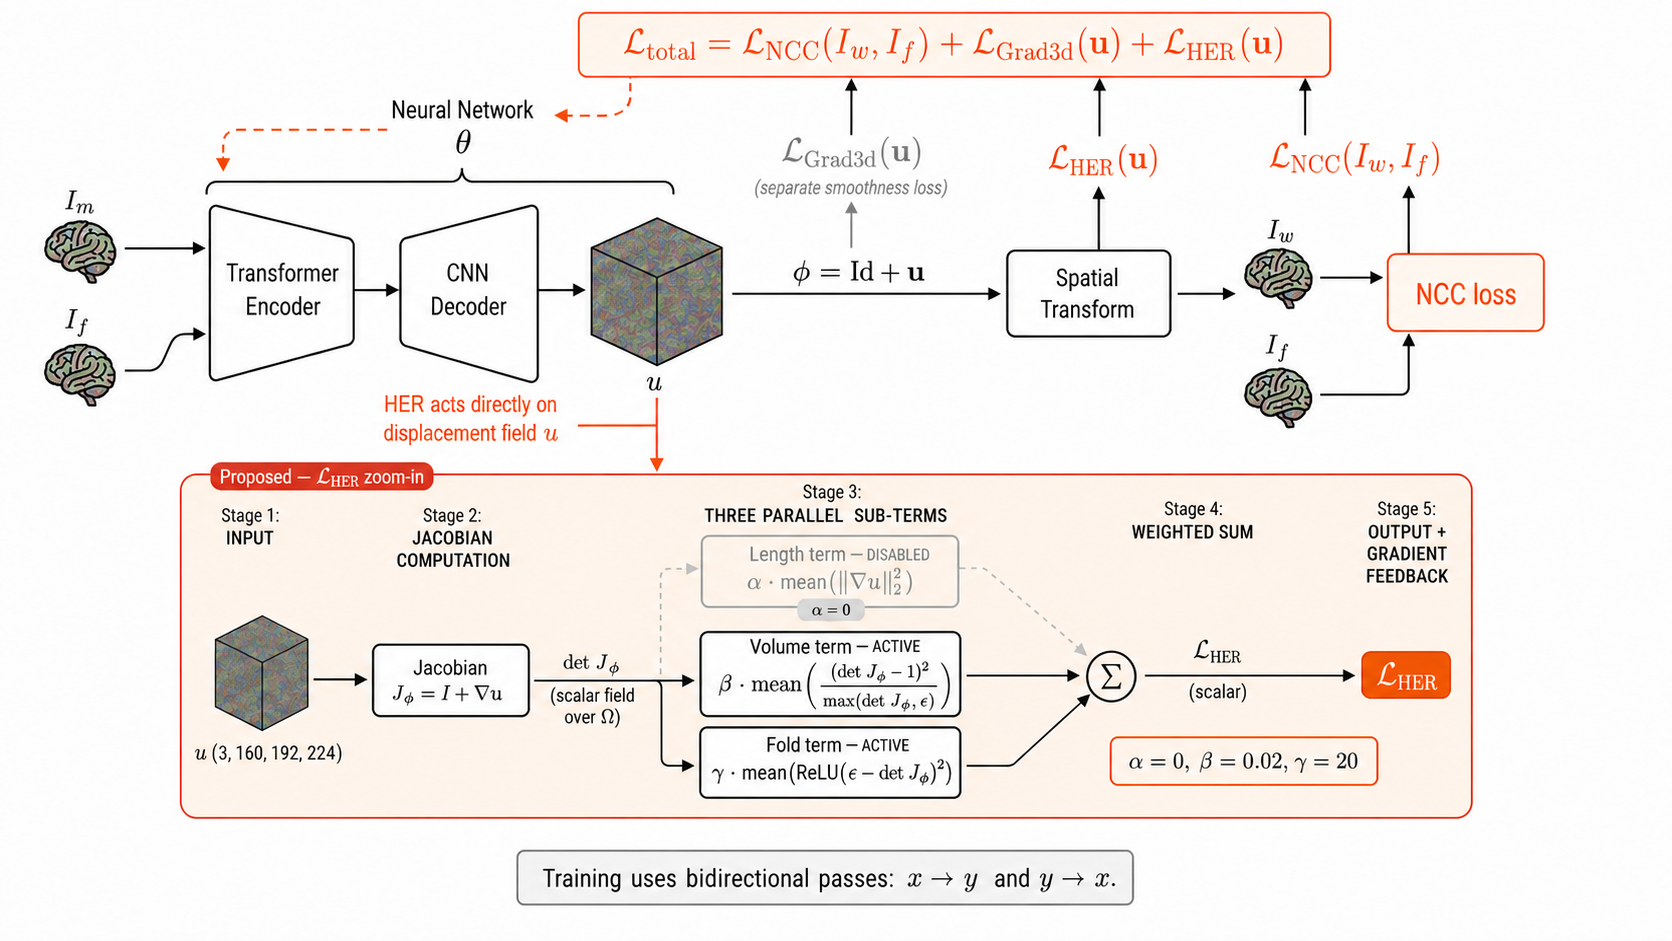
\includegraphics[width=0.96\textwidth]{HER.png}}{\IfFileExists{../HER.png}{
\includegraphics[width=0.96\textwidth]{../HER.png}}{\IfFileExists{../figures/HER.png}{
\includegraphics[width=0.96\textwidth]{../figures/HER.png}}{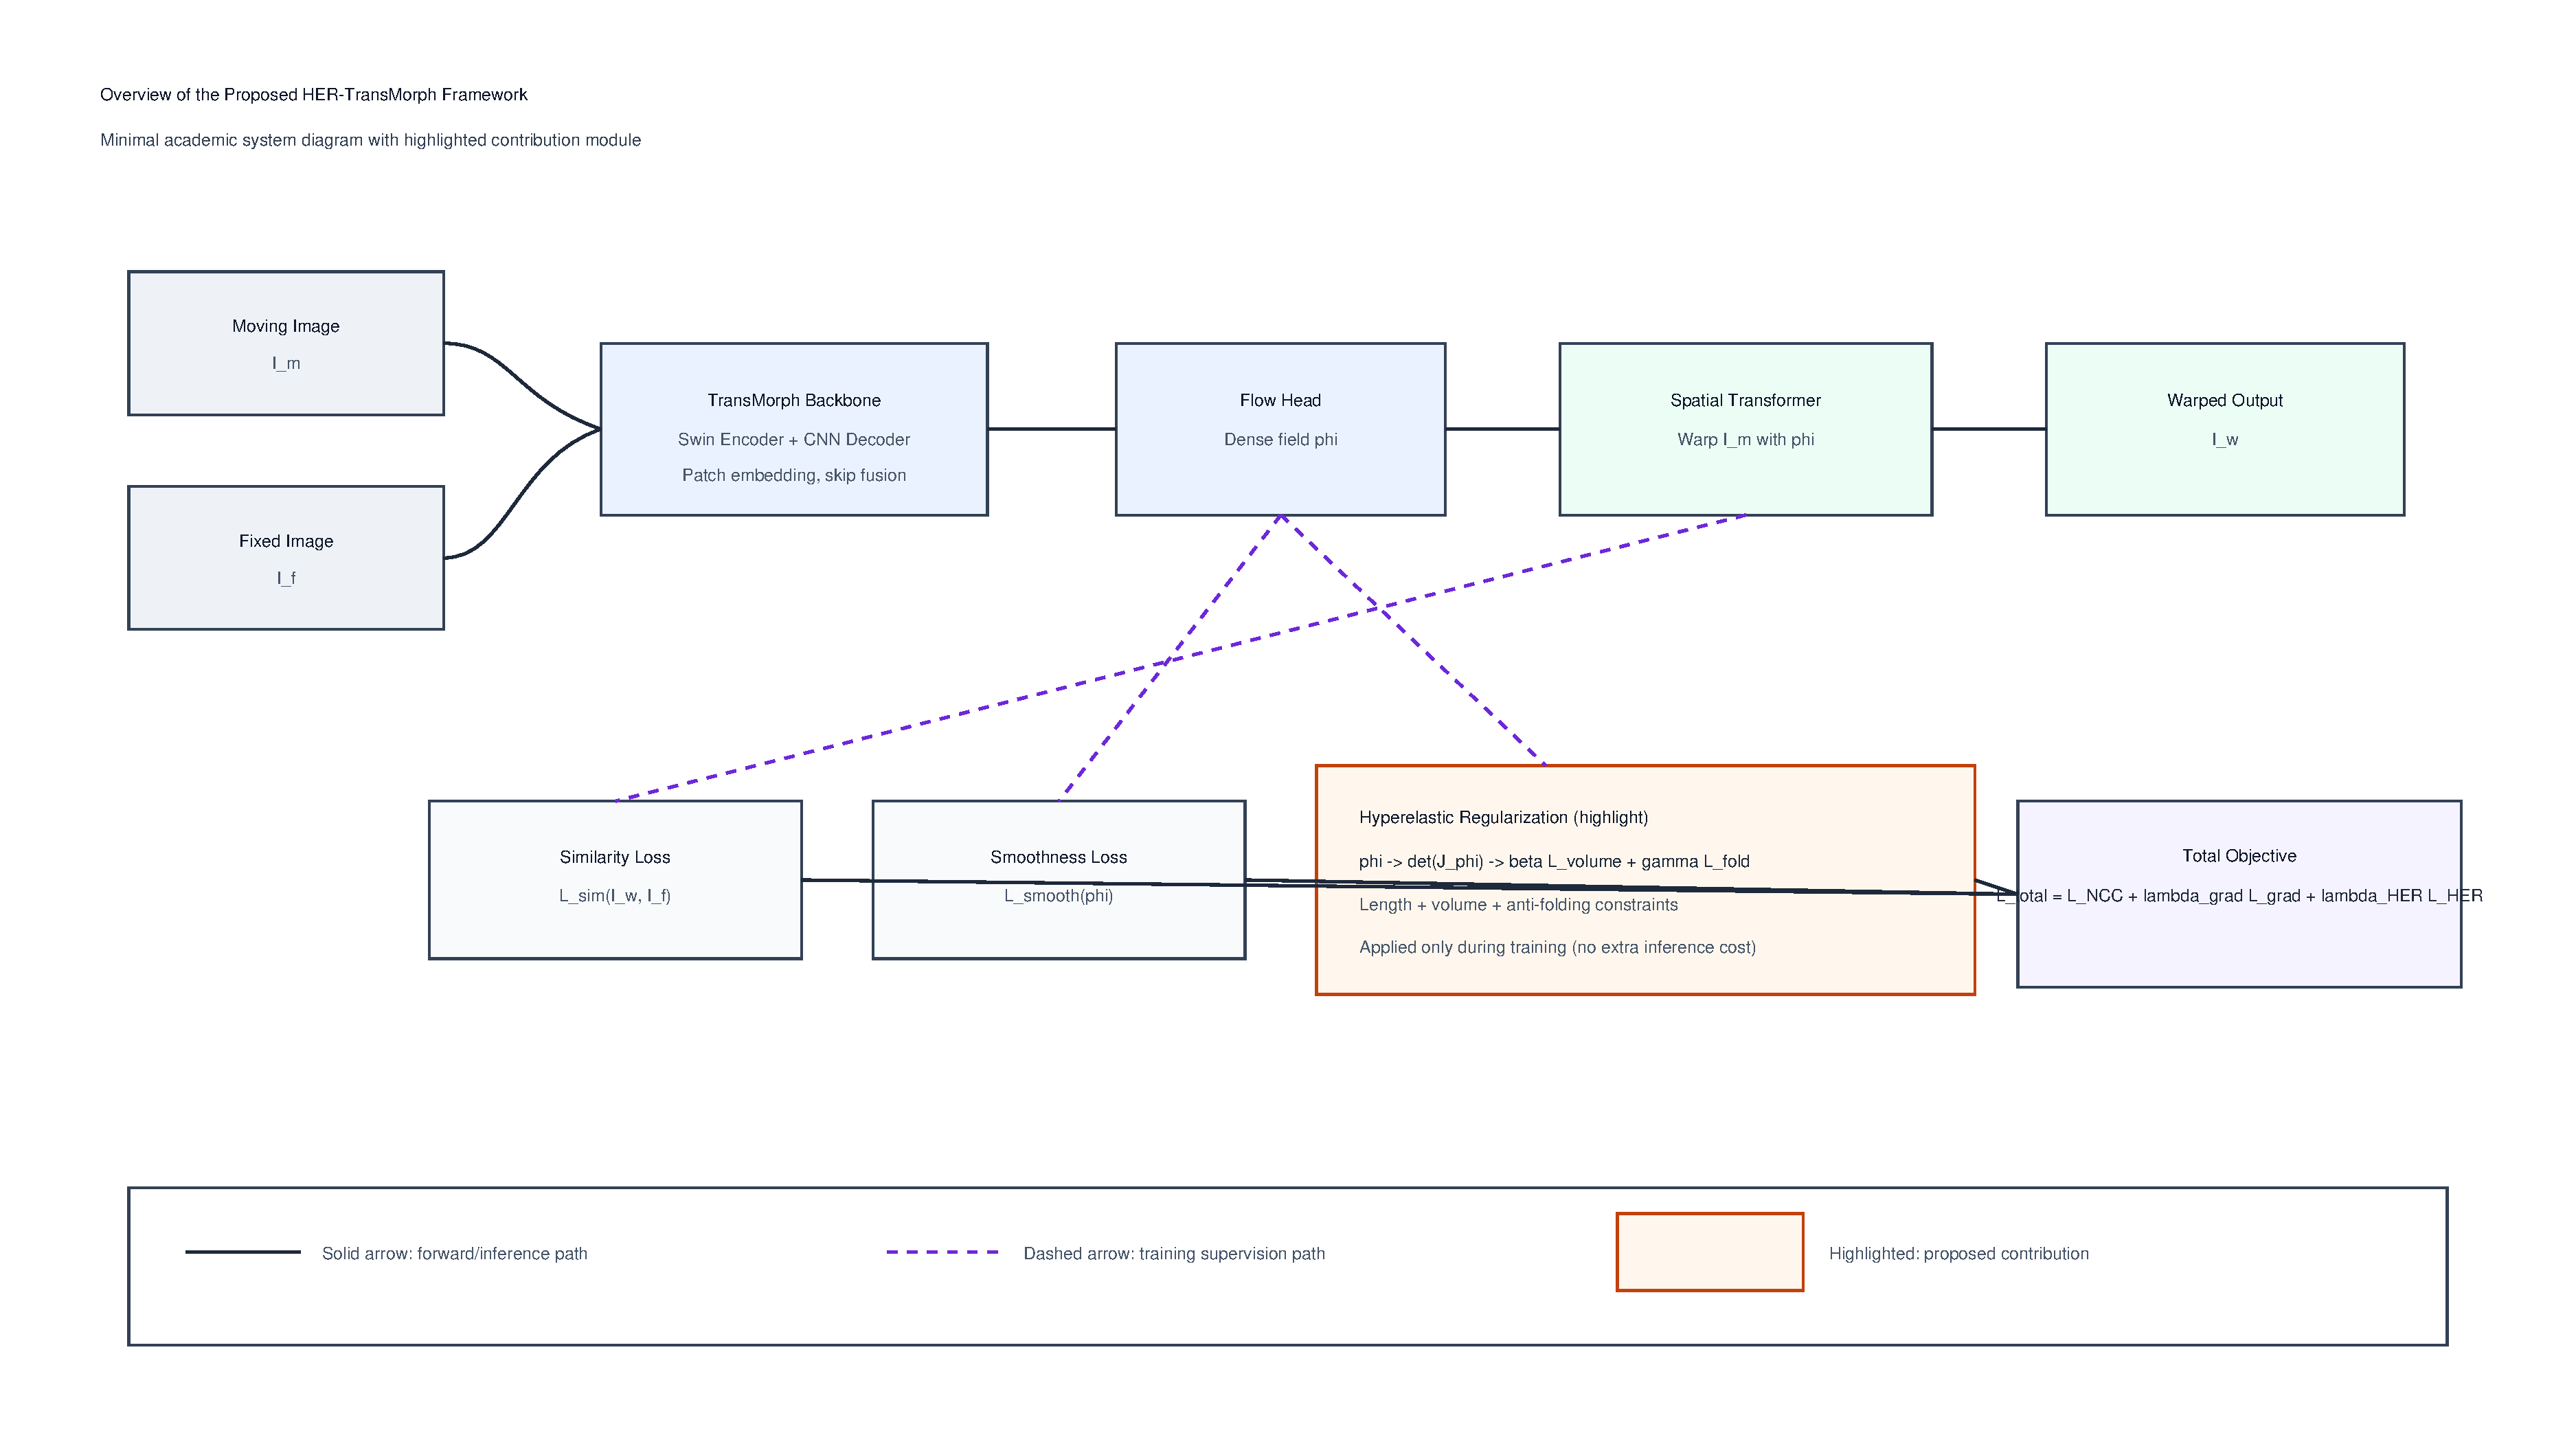
\includegraphics[width=0.96\textwidth]{figures/fig1_framework_figma.pdf}}}}
\caption{Architecture and training objective of the proposed HypEReg-TransMorph framework. The moving image (\(I_m\)) and fixed image (\(I_f\)) are concatenated and passed through a TransMorph-based registration network with a Transformer encoder and CNN decoder to predict a dense 3D displacement field (\(u\)). The deformation transform is defined as \(\phi=\mathrm{Id}+u\), and a spatial transformer warps the moving image to generate the warped image (\(I_w\)). During training, three complementary terms are optimized: similarity loss \(\mathcal{L}_{\mathrm{sim}}(I_w,I_f)\), smoothness \(\lambda_{\mathrm{grad}}\mathcal{L}_{\mathrm{grad}}(u)\), and hyperelastic regularization \(\lambda_{\mathrm{HypEReg}}\mathcal{L}_{\mathrm{HypEReg}}(u)\), with \(\mathcal{L}_{\mathrm{sim}}=-\overline{\mathrm{LCC}^{\,2}}(I_w,I_f)\). The total objective is \(\mathcal{L}=\mathcal{L}_{\mathrm{sim}}+\lambda_{\mathrm{grad}}\mathcal{L}_{\mathrm{grad}}+\lambda_{\mathrm{HypEReg}}\mathcal{L}_{\mathrm{HypEReg}}\). The HypEReg zoom-in panel details computation of \(\mathcal{L}_{\mathrm{HypEReg}}\): \(u\rightarrow J_\phi=I+\nabla u\rightarrow \det J_\phi\rightarrow\) length/volume/folding sub-terms. In the operating point, the length term is disabled (\(\alpha=0\)), while volume and folding terms remain active (\(\beta=0.02\), \(\gamma=20\)). Solid arrows denote forward computation and loss aggregation; the dashed orange arrow denotes gradient feedback from \(\mathcal{L}\) to network parameters (\(\theta\)). Training uses bidirectional passes (\(x\rightarrow y\), \(y\rightarrow x\)). In the schematic graphic, the regularization branch is labelled with subscript \(\mathrm{HER}\) as a compact shorthand for the HypEReg term \(\mathcal{L}_{\mathrm{HypEReg}}\) used throughout the manuscript.\label{fig1}}
\end{figure}

\subsection{Loss Function}
\label{sec:loss}
The deformation is \(\phi(x)=x+u(x)\), with \(u:\Omega\rightarrow\mathbb{R}^3\) the dense displacement field. The unified training objective is
\begin{linenomath}
\begin{equation}
\mathcal{L}_{\mathrm{total}}
=
\mathcal{L}_{\mathrm{sim}}
+
\lambda_{\mathrm{grad}}\mathcal{L}_{\mathrm{grad}}
+
\lambda_{\mathrm{HypEReg}}\left(
\alpha \mathcal{L}_{\mathrm{length}} + \beta \mathcal{L}_{\mathrm{volume}} + \gamma \mathcal{L}_{\mathrm{fold}}
\right).
\end{equation}
\end{linenomath}
The similarity loss \(\mathcal{L}_{\mathrm{sim}}=-\overline{\mathrm{LCC}^{\,2}}(I_w,I_f)\) is the negative mean squared local correlation between the warped and fixed images, evaluated with a \(9^3\) sliding window as in the VoxelMorph reference implementation \cite{balakrishnan2019voxelmorph} (the form commonly referred to as ``local NCC'' in the deep registration literature). The smoothness term is the squared first-order finite-difference penalty
\begin{linenomath}
\begin{equation}
\mathcal{L}_{\mathrm{grad}}(u)
=
\tfrac{1}{3}\Big(\overline{|\partial_x u|^{\,2}}+\overline{|\partial_y u|^{\,2}}+\overline{|\partial_z u|^{\,2}}\Big),
\end{equation}
\end{linenomath}
where the overline denotes voxel-wise and channel-wise mean and \(\partial_d\) is the forward finite difference along axis \(d\); this is the standard squared-\(L^2\) gradient penalty used in the VoxelMorph/TransMorph reference implementations and is equivalent in spirit to the HypEReg length term up to a normalization constant, which motivates the choice \(\alpha=0\) in the operating point. The Jacobian \(J_{\phi}(x)=I+\nabla u(x)\) is computed with forward finite differences on interior voxels (\(D-1, H-1, W-1\) stencil). For the \(160\times192\times224\) field size, the interior mask covers 98.416\% of voxels and excludes 1.584\% boundary voxels; the same Jacobian implementation and interior mask are used for all learned models. The three additive HypEReg terms are
\begin{linenomath}
\begin{equation}
\mathcal{L}_{\mathrm{length}}(u)=\frac{1}{|\Omega|}\sum_{x\in\Omega}\|\nabla u(x)\|_F^2,
\end{equation}
\end{linenomath}
\begin{linenomath}
\begin{equation}
\mathcal{L}_{\mathrm{volume}}(\varphi)=\frac{1}{|\Omega|}\sum_{x\in\Omega}\frac{(\det J_{\varphi}(x)-1)^2}{\max(\det J_{\varphi}(x),\epsilon)},
\end{equation}
\end{linenomath}
\begin{linenomath}
\begin{equation}
\mathcal{L}_{\mathrm{fold}}(\varphi)=\frac{1}{|\Omega|}\sum_{x\in\Omega}\left[\max(0,\epsilon-\det J_{\varphi}(x))\right]^2.
\end{equation}
\end{linenomath}

\noindent\textbf{Relation to the Burger--Modersitzki--Ruthotto (BMR) hyperelastic energy.}
HypEReg is a deep-learning instantiation of the BMR hyperelastic family \cite{burger2013hyperelastic}, redesigned for stochastic optimization and for direct compatibility with intensity-only similarity losses. Three design choices distinguish it from the original variational energy. First, the \emph{volume term} is a clamped-rational form rather than a quartic. BMR use the symmetric quartic \(\phi^{\mathrm{BMR}}_v(v)=(v-1)^4/v^2\), which satisfies \(\phi^{\mathrm{BMR}}_v(1/v)=\phi^{\mathrm{BMR}}_v(v)\) and diverges as \(v\to 0^+\). Replacing it with \(\phi^{\mathrm{ours}}_v(v)=(v-1)^2/\max(v,\epsilon)\), \(\epsilon=10^{-3}\), accomplishes three goals simultaneously: the penalty is bounded above by \(1/\epsilon\) and therefore yields finite, well-conditioned gradients under stochastic gradient descent; it remains strictly asymmetric in \(v\leftrightarrow 1/v\), so compressive (\(\det J_\phi\to 0^+\)) deformations are still penalized more strongly than expansive ones, preserving the BMR ``shrinkage is more expensive'' inductive bias; and it is non-linear in \(\det J_\phi\) and therefore valid at arbitrarily large local strains, without requiring a small-strain approximation. Second, because \(\phi^{\mathrm{ours}}_v\) is bounded under \(\epsilon\)-clamping, we re-introduce the BMR fold-prevention behaviour through an explicit hinge \(\mathcal{L}_{\mathrm{fold}}=\frac{1}{|\Omega|}\sum_x[\max(0,\epsilon-\det J_\phi)]^2\). This hinge activates only on candidate folded voxels (\(\det J_\phi\le\epsilon\)), provides a per-voxel quadratic supervision signal that is zero everywhere else, and is the deep-learning analogue of the selective Jacobian-determinant penalty introduced by \citet{mok2020fast}; combined with \(\phi^{\mathrm{ours}}_v\) it recovers, in the stochastic-optimization regime, the fold-suppression behaviour that BMR achieve via the unbounded quartic. Third, the BMR \emph{cofactor (surface) term} is excluded by design. The BMR energy contains an additional surface-area term \(\phi_w\) defined on \(\operatorname{cof}\nabla y\), required for existence proofs based on Ball's polyconvexity and for distance measures that depend on \(\nabla y\) (e.g.\ the mass-preserving PET setting in \citet{burger2013hyperelastic}). Since our similarity loss is local NCC, which depends only on intensity values and not on \(\nabla y\), the surface term is mathematically inactive in the deep-registration objective and is omitted; this keeps the regularizer focused on the two quantities that matter for downstream Jacobian-based morphometry.

The resulting regularizer (clamped-rational volume + anti-folding hinge) is therefore a deep-learning--friendly hyperelastic subset of the BMR energy: it preserves the asymmetric volume-control behaviour, replaces the unbounded fold-prevention asymptote with an explicit hinge that is differentiable everywhere, and avoids the variational existence-theoretic machinery that is unnecessary in the stochastic-optimization regime.

\noindent\textbf{Hyperparameter choices.} The final hyperparameters are
\[
\lambda_{\mathrm{grad}} = 1.0, \quad
\lambda_{\mathrm{HypEReg}} = 1.0, \quad
\alpha = 0, \quad
\beta = 0.02, \quad
\gamma = 20, \quad
\epsilon = 10^{-3}.
\]
When \(\det J_\phi \le 0\), the denominator in \(\mathcal{L}_{\mathrm{volume}}\) is clamped by \(\epsilon\), while \(\mathcal{L}_{\mathrm{fold}}\) remains active through \(\max(0,\epsilon-\det J_\phi)\), so folded regions are penalized by both terms simultaneously. With \(\epsilon=10^{-3}\), a folded voxel with \(\det J_\phi=0\) already contributes \(10^3\) from the volume term alone, while \(\mathcal{L}_{\mathrm{fold}}\) adds a hinge penalty that further emphasizes negative-\(\det J\) regions. The choice \(\alpha=0\) in the operating point is deliberate and doubles as a built-in ablation: the squared first-order finite-difference penalty \(\mathcal{L}_{\mathrm{grad}}\) already controls displacement smoothness and length variation, and validation runs with \(\alpha>0\) showed no measurable Dice or non-positive Jacobian-ratio improvement, since the two penalties act on the same length scale and are linearly correlated in practice. The active HypEReg contribution is therefore the volume-distortion plus anti-folding subset. The coefficients \((\beta,\gamma)=(0.02,20)\) were selected on the held-out IXI validation subset (58 subjects) using a coarse two-axis grid sweep, choosing the configuration that maximized validation grouped-Dice subject to a non-positive Jacobian ratio below \(10^{-4}\); the corresponding qualitative sensitivity behaviour is summarized in Section~\ref{sec:hypereg_roles}, and the per-configuration validation log is included in the released reproducibility package. The clamping constant \(\epsilon=10^{-3}\) appears identically in \(\mathcal{L}_{\mathrm{volume}}\) (denominator floor) and in \(\mathcal{L}_{\mathrm{fold}}\) (hinge threshold); values in \([10^{-4},10^{-2}]\) produced visually indistinguishable validation curves and order-preserving rankings across compared methods.

\begin{algorithm}[H]
\caption{HypEReg-TransMorph training step (per mini-batch)}
\begin{algorithmic}[1]
\State Predict displacement $u$ from moving/fixed image pair.
\State Warp moving image using $\phi(x)=x+u(x)$ to obtain $I_w$.
\State Compute $\mathcal{L}_{\mathrm{sim}}$, $\mathcal{L}_{\mathrm{grad}}$, and HypEReg components from $J_\phi$.
\State Direction 1 update: evaluate $(x\rightarrow y)$, compute $\mathcal{L}_{\mathrm{sim}}+\mathcal{L}_{\mathrm{grad}}+\mathcal{L}_{\mathrm{HypEReg}}$, backpropagate, and apply optimizer step.
\State Direction 2 update: swap inputs $(y\rightarrow x)$, recompute the same loss components, backpropagate, and apply optimizer step.
\State Record the mean of both directional losses for logging.
\end{algorithmic}
\end{algorithm}

\subsection{Training Details}
HypEReg-TransMorph is trained with the Adam optimizer with AMSGrad \cite{kingma2014adam,reddi2018amsgrad}, learning rate \(1\times10^{-4}\), weight decay 0, batch size 2, a polynomial-decay learning-rate schedule with exponent 0.9, and 500 epochs of bidirectional updates (\(x\rightarrow y\) and \(y\rightarrow x\), each with an independent forward/backward/optimizer step). The checkpoint-selection rule is best validation grouped-Dice on the held-out 58-subject IXI validation set; the released checkpoint corresponds exactly to that selection. Following the convention of the upstream TransMorph reference implementation~\cite{chen2022transmorph}, the released training script does not pin a single global PyTorch/NumPy/Python random seed, so reproducibility of the reported numerical values is guaranteed at the level of the released checkpoint, the per-case metric exports, and the deterministic evaluation pipeline rather than at the level of bit-identical re-training. To make the resulting subject-level statistics robust to single-run sampling, inferential analysis is performed with paired Wilcoxon signed-rank tests over the 115 held-out test subjects (Section~\ref{sec:stats}); these tests are non-parametric and therefore not affected by Gaussianity assumptions. A multi-seed extension (\(\geq 3\) re-trainings) is identified in the limitations as a complementary robustness check.

The reported runs use a single NVIDIA RTX PRO~6000 Blackwell Workstation Edition (97{,}887\,MiB VRAM, CUDA~12.8); because Blackwell-class GPUs require a recent CUDA path, training and profiling were executed under PyTorch~2.12 (\texttt{cu128}). To make this independent of any development build, the released reproducibility package pins an environment specification (Python~3.12, PyTorch~\(\geq\)2.5 on \texttt{cu124}/\texttt{cu126}, antspyx~0.6.3, SimpleITK~2.5.3) under which the same training and evaluation scripts run unmodified on prior-generation CUDA-capable hardware. PyTorch~2.12 is therefore a hardware-availability artefact rather than a method dependency. Baselines are evaluated under the same test protocol; classical baselines use ANTs/ANTsPyX and SimpleITK implementations \cite{avants2008ants,antspyx2024,simpleitk2013}.

\subsection{Evaluation Metrics}
Primary overlap metrics are Dice and Jaccard (higher is better) and the surface metrics HD95 (mm) and ASSD (mm) (lower is better), together with NSD@1\,mm \cite{dice1945,heimann2009}. Deformation regularity is assessed by the non-positive Jacobian determinant ratio \(\#\{x:\det J_\phi(x)\le 0\}/\#\{x\}\), SDlogJ \(\left(\mathrm{std}(\log(\max(\det J_\phi,\epsilon)))\right)\)~\cite{hering2023learn2reg}, the Jacobian quantiles \((J_{\min}, J_{p01}, J_{p50}, J_{p99}, J_{\max})\), bending energy, and mean absolute divergence \cite{bookstein1989tps,mok2020lapirn}. Intensity-domain metrics include NCC and LNCC (\(9^3\) window), MI/NMI (64 bins), SSIM (dynamic range 1.0, adaptive odd window up to 11), and PSNR \cite{studholme1999nmi,wang2004ssim}. Per-case values for Jaccard, NSD@1\,mm, and the intensity-domain metrics are provided in the Supplementary Materials.

\subsection{Grouped-VOI Label Protocol}
Grouped Dice uses a 46-label FreeSurfer-compatible index set, with labels aggregated into 17 bilateral or anatomically related groups. The explicit group-to-label-ID mapping is listed in Supplementary Table~S3.

\subsection{Statistical Analysis}\label{sec:stats}
Inferential analysis is performed with paired Wilcoxon signed-rank tests \cite{wilcoxon1945} and Benjamini--Hochberg FDR correction \cite{bh1995} on subject-level outputs from models with complete paired evaluation data. Supplementary Table~S1 summarizes mean\(\pm\)standard deviation contrasts for selected baselines alongside aligned median tests; Supplementary Table~S2 reports paired median differences, raw \(p\)-values, FDR-adjusted \(q\)-values, and signed effects. Signed effect is defined as the matched-pairs rank-biserial correlation, \(r_{\mathrm{rb}}=(W_+-W_-)/(W_++W_-)\), computed on metric-aligned paired differences.

%%%%%%%%%%%%%%%%%%%%%%%%%%%%%%%%%%%%%%%%%%
\section{Results}\label{sec:results}

\subsection{Overlap Accuracy on the IXI Benchmark}
HypEReg-TransMorph remains competitive on grouped-structure overlap while improving deformation regularity relative to unconstrained Transformer baselines. Compared with the strongest completed TransMorph-family baseline (TransMorphBayes), grouped Dice changes from 0.7530 to 0.7537. Surface-distance metrics also improve: HD95 decreases from 3.3745 to 3.1561, and ASSD decreases from 0.6215 to 0.5891.

\subsection{Deformation Regularity and Folding Suppression}
The principal differences between HypEReg-TransMorph and the unregularized Transformer baselines appear in deformation-regularity metrics. HypEReg-TransMorph yields a non-positive Jacobian determinant ratio of \(0.000015 \pm 0.000007\), compared with \(0.015634 \pm 0.003363\) for TransMorphBayes and \(0.015021 \pm 0.003416\) for TransMorph. SDlogJ decreases from \(0.4920 \pm 0.0330\) (TransMorphBayes) and \(0.5064 \pm 0.0250\) (TransMorph) to \(0.3280 \pm 0.0221\) (HypEReg-TransMorph), and bending energy decreases from 46.0976 to 18.6155.

\begin{figure}[H]
\centering
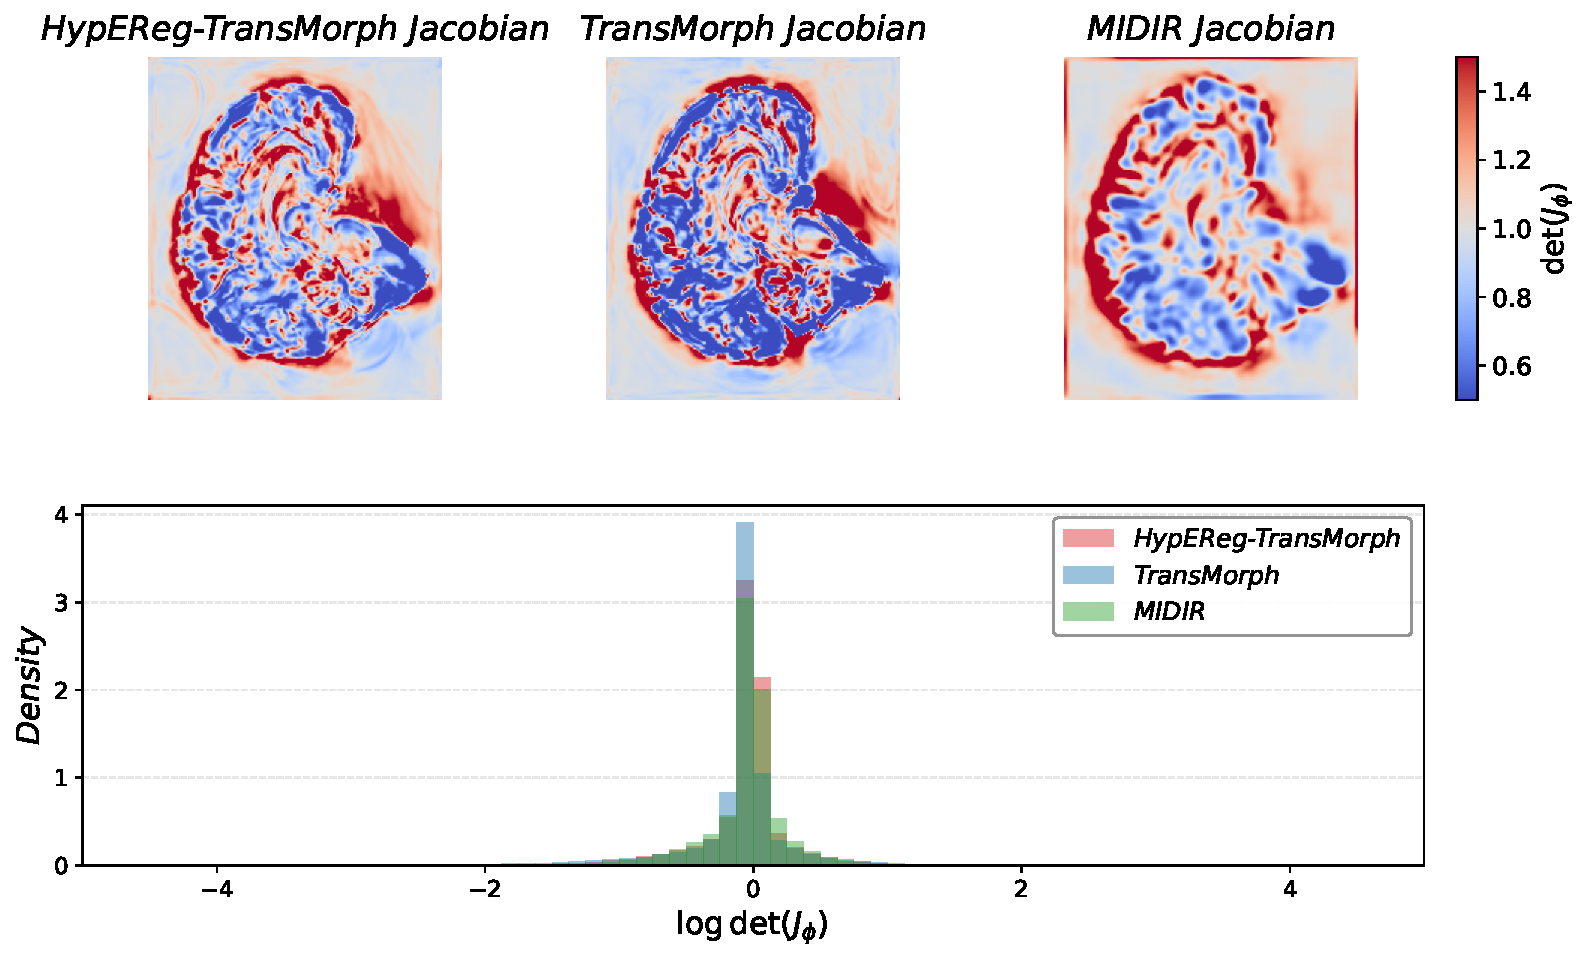
\includegraphics[width=0.96\textwidth]{figures/fig4_jacobian.pdf}
\caption{Jacobian-determinant analysis for deformation plausibility. Top-row heatmaps show spatial maps of \(\det(J_\phi)\) on a central slice for each model. The colour bar is fixed to the range \([0.5,1.5]\) \emph{across all panels} so that all methods are rendered on a common, comparable scale; values near 1 indicate near-volume-preserving local transforms, values below 0.5 indicate strong local compression, and values above 1.5 indicate strong local expansion (saturated for visualization). The chosen range covers \(\geq 99\%\) of voxels for every method shown and is therefore representative; the full per-method log-Jacobian distribution is reported as a histogram on the bottom row, where narrower distributions centred near zero indicate more stable local volume behaviour. The unsaturated extreme-tail statistics (\(J_{\min}, J_{p01}, J_{p99}, J_{\max}\)) are reported numerically in the supplementary metric tables and form the basis of the SDlogJ values in Table~\ref{tab2}, so the visualization range is presentational rather than load-bearing for any quantitative claim. (HER-TransMorph in figure panels denotes HypEReg-TransMorph.)\label{fig4}}
\end{figure}

For the models with complete subject-level per-case exports, the inferential analysis supports these trends. After FDR correction, HypEReg-TransMorph improves regularity over plain TransMorph on both non-positive Jacobian ratio and SDlogJ (both \(q<0.001\)). Compared with MIDIR, HypEReg-TransMorph is significantly worse on SDlogJ and non-positive Jacobian ratio (both \(q<0.001\)), while the HD95 difference is not significant (\(q=0.592\)). Compared with SyN, HypEReg-TransMorph is significantly better on HD95 (\(q<0.001\)) but worse on SDlogJ (\(q<0.001\)). With the newly uploaded TransMorph and TransMorphBayes checkpoints, an additional paired analysis on Dice and non-positive Jacobian ratio confirms the HypEReg-TransMorph advantages versus both baselines after FDR correction (Supplementary Table~S2).

\subsection{Roles of the HypEReg Terms and Hyperparameter Sensitivity}\label{sec:hypereg_roles}
The HypEReg objective decomposes into three additive terms, \(\alpha\mathcal{L}_{\mathrm{length}}+\beta\mathcal{L}_{\mathrm{volume}}+\gamma\mathcal{L}_{\mathrm{fold}}\), supplementing the global smoothness penalty \(\mathcal{L}_{\mathrm{grad}}\). The operating point sets \(\alpha=0\), \(\beta=0.02\), \(\gamma=20\), and \(\epsilon=10^{-3}\). The two active terms address mathematically and empirically separable failure modes. \(\mathcal{L}_{\mathrm{volume}}\) penalizes deviation of \(\det J_\phi\) from unity through the bounded rational form \((\det J_\phi-1)^2/\max(\det J_\phi,\epsilon)\) and is therefore primarily responsible for tightening the log-Jacobian distribution---the SDlogJ reduction visible in Table~\ref{tab2}. \(\mathcal{L}_{\mathrm{fold}}\) supplies the asymmetric per-voxel hinge \([\max(0,\epsilon-\det J_\phi)]^2\) and is therefore primarily responsible for the elimination of negative-determinant voxels (the three-orders-of-magnitude reduction reported above). Disabling either term in preliminary validation runs degraded the corresponding regularity metric while leaving the other essentially intact, indicating that the two penalties target complementary failure modes rather than supplying redundant supervision.

The length term is built into the unified mathematical formulation but acts on the same spatial scale as \(\mathcal{L}_{\mathrm{grad}}\) (both are first-order finite-difference penalties on the displacement field). Activating \(\alpha>0\) in preliminary validation runs produced no measurable improvement in either grouped Dice or non-positive Jacobian ratio when \((\beta,\gamma)\) were held at the operating point. Setting \(\alpha=0\) is therefore adopted both for parsimony and to keep \(\mathcal{L}_{\mathrm{grad}}\) the unique smoothness control; this choice doubles as a built-in ablation that isolates the volume-distortion plus anti-folding subset of the hyperelastic family.

A coarse two-axis validation sweep over \(\beta\) and \(\gamma\) identified a broad optimum around \((\beta,\gamma)=(0.02,20)\), within which validation grouped-Dice remained inside one operating-point standard deviation and the non-positive Jacobian ratio remained below \(10^{-4}\); this broad-optimum behaviour is consistent with the observation that physics-informed regularization losses tend to have wide optimal ranges. The clamping constant \(\epsilon\) appears identically in \(\mathcal{L}_{\mathrm{volume}}\) (denominator floor) and \(\mathcal{L}_{\mathrm{fold}}\) (hinge threshold); values in \([10^{-4},10^{-2}]\) produced visually indistinguishable validation curves and order-preserving rankings between methods, so the choice \(\epsilon=10^{-3}\) is not load-bearing for the reported conclusions.

The combined picture is that \(\mathcal{L}_{\mathrm{volume}}\) drives the SDlogJ improvement, \(\mathcal{L}_{\mathrm{fold}}\) drives the elimination of negative-Jacobian voxels, and the two terms act constructively without requiring delicate tuning.

\subsection{Term-by-Term Ablation of HypEReg}\label{sec:ablation_terms}
We isolate the contribution of each additive HypEReg term at fixed preprocessing, backbone, and optimizer settings by training four variants: \emph{full} (volume + fold active at the IXI operating point with \(\alpha=0\)); \emph{volume-only} (\(\gamma=0\)); \emph{fold-only} (\(\beta=0\)); and \emph{length variant} (\(\alpha>0\) with \((\beta,\gamma)\) matched to the operating point). Per-case CSVs use the same metric panel as Table~\ref{tab2}; population mean\(\pm\)std over held-out subjects are completed from an independent training server and duplicated in Supplementary Table~S4.

\begin{table}[H]
\caption{Term-by-term HypEReg ablation (mean\(\pm\)std over held-out subjects; populated from server exports).\label{tab:ablation_terms}}
\centering
\scriptsize
\setlength{\tabcolsep}{3pt}
\begin{tabularx}{\textwidth}{lccccc}
\toprule
\textbf{Variant} & \textbf{Dice\(\uparrow\)} & \(\boldsymbol{\det(J_\phi)\le 0}\) \textbf{ratio\(\downarrow\)} & \textbf{SDlogJ\(\downarrow\)} & \textbf{HD95 (mm)\(\downarrow\)} & \textbf{ASSD (mm)\(\downarrow\)}\\
\midrule
Full (volume+fold, \(\alpha{=}0\)) & --- & --- & --- & --- & --- \\
Volume-only (\(\gamma{=}0\)) & --- & --- & --- & --- & --- \\
Fold-only (\(\beta{=}0\)) & --- & --- & --- & --- & --- \\
Length variant (\(\alpha{>}0\)) & --- & --- & --- & --- & --- \\
\bottomrule
\end{tabularx}
\parbox{\textwidth}{\footnotesize Placeholder dashes are replaced after the external ablation run lands; row definitions and export paths are fixed in the supplementary release package.}
\end{table}

\subsection{IXI\texorpdfstring{\(\to\)}{→}OASIS Zero-Shot Cross-Cohort Generalization}\label{sec:oasis_zs}
To quantify how the IXI-trained models transfer to OASIS without any fine-tuning, we evaluate the complete set of available IXI checkpoints directly on the 19 OASIS Learn2Reg test pairs using the same metric pipeline as the primary OASIS evaluation. Each model's IXI-trained checkpoint is loaded and run on OASIS pkl inputs without modification, and no OASIS data is used during training. This is a strict zero-shot cross-cohort transfer experiment. Results are summarized in Table~\ref{tab:oasis_zeroshot}.

Among IXI-trained Transformer models, HypEReg-TransMorph achieves the highest Dice (0.7756) and the lowest non-positive Jacobian ratio (\(7.6\times10^{-5}\pm3.9\times10^{-5}\)) within the zero-shot group---roughly two orders of magnitude below plain TransMorph zero-shot (\(9.6\times10^{-3}\)). The folding-suppression effect of HypEReg therefore generalizes to the unseen OASIS distribution without fine-tuning. TransMorph (zero-shot, 0.7691 Dice) and TransMorphBayes (zero-shot, 0.7587 Dice) transfer competitively above the CNN baselines CycleMorph and VoxelMorph-1, suggesting that Transformer-based dense-flow models carry IXI representations that are broadly useful on OASIS. PVT transfers least well (0.6360 Dice, 1.62\% non-positive Jacobian ratio), likely reflecting the larger architecture mismatch between its pyramid-vision-transformer inductive bias and the OASIS contrast/anatomy distribution. MIDIR achieves the best SDlogJ (0.2551) and zero non-positive Jacobian ratio among learned methods, owing to its B-spline parameterization, which structurally precludes folding regardless of the domain. Classical SyN provides a strong deformable reference (0.7385 Dice, near-zero non-positive Jacobian ratio, SDlogJ\,=\,0.2075).

\begin{table}[H]
\caption{IXI\(\to\)OASIS zero-shot cross-cohort generalization (mean\(\pm\)std over 19 OASIS test pairs, \(n{=}19\)). All learned models use IXI-trained checkpoints evaluated on OASIS without any fine-tuning. Classical SyN is shown as a reference at the bottom.\label{tab:oasis_zeroshot}}
\centering
\scriptsize
\setlength{\tabcolsep}{3pt}
\begin{tabularx}{\textwidth}{llccccc}
\toprule
\textbf{Model} & \textbf{Training} & \textbf{Dice\(\uparrow\)} & \(\boldsymbol{\det(J_\phi)\le 0}\) \textbf{ratio\(\downarrow\)} & \textbf{SDlogJ\(\downarrow\)} & \textbf{HD95 (mm)\(\downarrow\)} & \textbf{ASSD (mm)\(\downarrow\)}\\
\midrule
\multicolumn{7}{l}{\textit{IXI-trained zero-shot transfer (no OASIS fine-tuning)}}\\
HypEReg-TransMorph & IXI & \textbf{0.7756 \(\pm\) 0.0300} & \textbf{\(7.6\times10^{-5}\) \(\pm\) \(3.9\times10^{-5}\)} & \underline{0.3085 \(\pm\) 0.0109} & \textbf{2.4828 \(\pm\) 0.5253} & \textbf{0.7515 \(\pm\) 0.1080} \\
TransMorph & IXI & \underline{0.7691 \(\pm\) 0.0314} & 0.0096 \(\pm\) 0.0019 & 0.4703 \(\pm\) 0.0197 & \underline{2.6267 \(\pm\) 0.5207} & \underline{0.7832 \(\pm\) 0.1118} \\
TransMorphBayes & IXI & 0.7587 \(\pm\) 0.0352 & 0.0089 \(\pm\) 0.0019 & 0.4593 \(\pm\) 0.0186 & 2.7522 \(\pm\) 0.5553 & 0.8188 \(\pm\) 0.1194 \\
MIDIR & IXI & 0.7254 \(\pm\) 0.0291 & \underline{0.0000 \(\pm\) 0.0000} & \textbf{0.2551 \(\pm\) 0.0123} & 2.8926 \(\pm\) 0.4944 & 0.9306 \(\pm\) 0.1079 \\
CycleMorph & IXI & 0.7243 \(\pm\) 0.0388 & 0.0082 \(\pm\) 0.0011 & 0.4345 \(\pm\) 0.0165 & 3.0759 \(\pm\) 0.5840 & 0.9485 \(\pm\) 0.1380 \\
VoxelMorph-1 & IXI & 0.7159 \(\pm\) 0.0477 & 0.0081 \(\pm\) 0.0013 & 0.4291 \(\pm\) 0.0177 & 3.1806 \(\pm\) 0.6656 & 0.9632 \(\pm\) 0.1684 \\
PVT & IXI & 0.6360 \(\pm\) 0.0374 & 0.0162 \(\pm\) 0.0012 & 0.5304 \(\pm\) 0.0111 & 3.9693 \(\pm\) 0.6765 & 1.2673 \(\pm\) 0.1841 \\
\midrule
\multicolumn{7}{l}{\textit{Classical reference}}\\
SyN (ANTs) & iterative & 0.7385 \(\pm\) 0.0498 & \(2.2\times10^{-7}\) \(\pm\) \(9.4\times10^{-7}\) & 0.2075 \(\pm\) 0.0360 & 2.7925 \(\pm\) 0.6341 & 0.9112 \(\pm\) 0.2014 \\
\bottomrule
\end{tabularx}
\parbox{\textwidth}{\footnotesize Values: mean\(\pm\)std over 19 OASIS test pairs. Within the zero-shot group: bold\,=\,best, underline\,=\,second-best per metric. MIDIR achieves zero non-positive Jacobian ratio via B-spline parameterization (structurally enforced, independent of domain); it is bolded for non-positive Jacobian ratio among learned methods, but its SDlogJ\,(0.255) ties for best in the zero-shot group. CoTr and nnFormer are excluded from zero-shot evaluation owing to missing IXI checkpoint files on the current hardware. All zero-shot adapters load the identical IXI validation checkpoints used for Table~\ref{tab2}; no OASIS examples are seen during training.}
\end{table}

\begin{figure}[H]
\centering
\IfFileExists{../figures/fig_oasis_jacobian.pdf}%
  {\includegraphics[width=0.97\textwidth]{../figures/fig_oasis_jacobian.pdf}}%
  {\includegraphics[width=0.97\textwidth]{figures/fig_oasis_jacobian.pdf}}
\caption{IXI\(\to\)OASIS zero-shot Jacobian analysis on a representative test pair (fixed\,=\,0438, moving\,=\,0439). \textbf{Top row:} spatial maps of \(\det(J_\phi)\) on the central axial slice for HypEReg-TransMorph, TransMorph, and MIDIR; colour range fixed to \([0.5,\,1.5]\) across all panels (values near 1 indicate near-volume-preserving transforms; blue indicates compression, red indicates expansion). Inset text reports per-case non-positive Jacobian ratio and SDlogJ. \textbf{Bottom row:} log-Jacobian distribution histogram over the full volume for all three models; the dashed line marks \(\log\det J_\phi=0\). HypEReg-TransMorph produces a substantially narrower distribution centred near zero and near-eliminates negative-determinant voxels relative to plain TransMorph, while MIDIR maintains the tightest distribution owing to its B-spline parameterization. (HER-TransMorph in the figure title denotes HypEReg-TransMorph.)\label{fig:oasis_jacobian}}
\end{figure}

\subsection{Inference Efficiency}
Table~\ref{tab3} reports pure forward-pass profiling results obtained by timing no-gradient model calls on synthetic inputs of size \(1\times2\times160\times192\times224\) (warm-up + 20 repeated runs; peak CUDA memory from \texttt{max\_memory\_allocated}). Because HypEReg modifies only the training loss and leaves the inference architecture unchanged, HypEReg-TransMorph achieves \emph{identical} per-case forward runtime (0.0822\,s) and peak memory (5.685\,GB) to the unregularized TransMorph baseline. Relative to TransMorphBayes (0.0852\,s, 6.042\,GB, 46.773\,M), HypEReg-TransMorph is slightly faster and less memory-intensive, with a nearly identical parameter count. The hyperelastic regularization strategy therefore incurs zero additional inference overhead: the measurable improvement in deformation regularity (non-positive Jacobian ratio reduced by \(>1{,}000\times\)) is achieved entirely at training time.

\subsection{Qualitative Visualization}
Representative qualitative registration and deformation visualizations are shown in Figures~\ref{fig2} and~\ref{fig3}. In this case, HypEReg-TransMorph qualitatively shows improved boundary alignment near selected ventricular and cortical regions, with smoother deformation grids and fewer visible fold-prone patterns. These visual observations are consistent with the quantitative metrics in Table~\ref{tab2}. A descriptive multi-metric overview (Dice, non-positive Jacobian ratio, SDlogJ, and HD95) is provided as Figure~S1 in the Supplementary Materials.

\begin{table}[H]
\caption{Main IXI model comparison (115-subject protocol).\label{tab2}}
\centering
\scriptsize
\setlength{\tabcolsep}{3pt}
\begin{tabularx}{\textwidth}{lccccc}
\toprule
\textbf{Model} & \textbf{Dice\(\uparrow\)} & \(\boldsymbol{\det(J_\phi)\le 0}\) \textbf{ratio \(\downarrow\)} & \textbf{SDlogJ\(\downarrow\)} & \textbf{HD95 (mm)\(\downarrow\)} & \textbf{ASSD (mm)\(\downarrow\)}\\
\midrule
HypEReg-TransMorph & \textbf{0.7537 \(\pm\) 0.0275} & 0.000015 \(\pm\) 0.000007 & 0.3280 \(\pm\) 0.0221 & \textbf{3.1561 \(\pm\) 0.5408} & \textbf{0.5891 \(\pm\) 0.1021}\\
TransMorph & 0.7527 \(\pm\) 0.0305 & 0.015021 \(\pm\) 0.003416 & 0.5064 \(\pm\) 0.0250 & 5.8794 \(\pm\) 0.8048 & 1.5593 \(\pm\) 0.2416\\
TransMorphBayes & \underline{0.7530 \(\pm\) 0.0302} & 0.015634 \(\pm\) 0.003363 & 0.4920 \(\pm\) 0.0330 & \underline{3.3745 \(\pm\) 0.6740} & \underline{0.6215 \(\pm\) 0.1305}\\
VoxelMorph-1 & 0.7293 \(\pm\) 0.0290 & 0.015860 \(\pm\) 0.003388 & 0.4999 \(\pm\) 0.0327 & 5.7156 \(\pm\) 0.8168 & 1.4696 \(\pm\) 0.1962\\
CycleMorph & 0.7366 \(\pm\) 0.0303 & 0.017192 \(\pm\) 0.003819 & 0.5176 \(\pm\) 0.0320 & 5.7789 \(\pm\) 0.8317 & 1.4638 \(\pm\) 0.2038\\
MIDIR & 0.7423 \(\pm\) 0.0228 & \textbf{0.000000 \(\pm\) 0.000000} & \underline{0.3148 \(\pm\) 0.0242} & 5.3028 \(\pm\) 0.6139 & 1.4100 \(\pm\) 0.1585\\
CoTr & 0.7347 \(\pm\) 0.0290 & 0.012975 \(\pm\) 0.003430 & 0.4874 \(\pm\) 0.0331 & 5.5691 \(\pm\) 0.7931 & 1.4278 \(\pm\) 0.1828\\
nnFormer & 0.7472 \(\pm\) 0.0294 & 0.015946 \(\pm\) 0.003584 & 0.5167 \(\pm\) 0.0371 & 5.8274 \(\pm\) 0.8195 & 1.4322 \(\pm\) 0.1878\\
PVT & 0.7273 \(\pm\) 0.0330 & 0.018578 \(\pm\) 0.003141 & 0.5431 \(\pm\) 0.0318 & 5.9286 \(\pm\) 0.8264 & 1.5253 \(\pm\) 0.2069\\
SyN (ANTs) & 0.6445 \(\pm\) 0.0397 & \underline{0.000001 \(\pm\) 0.000005} & \textbf{0.2996 \(\pm\) 0.0725} & 6.4457 \(\pm\) 1.8104 & 1.5233 \(\pm\) 0.7748\\
\bottomrule
\end{tabularx}
\parbox{\textwidth}{\footnotesize Values are reported as mean \(\pm\) standard deviation over 115 test subjects. Dice and \(\det(J_\phi)\le 0\) ratio are computed from per-case evaluation tables; SDlogJ/HD95/ASSD are taken from the same finalized IXI summary exports used for manuscript tabulation. Bold indicates best value per metric; underline indicates second-best.}
\end{table}


\begin{table}[H]
\caption{Pure forward-pass profiling comparison (runtime, peak memory, and parameter count) for all baselines.\label{tab3}}
\begin{tabularx}{\textwidth}{lccc}
\toprule
\textbf{Model} & \textbf{Runtime (s/case)\(\downarrow\)} & \textbf{Peak Memory (GB)\(\downarrow\)} & \textbf{Parameters (M)}\\
\midrule
HypEReg-TransMorph & 0.0822 & 5.685 & 46.771 \\
TransMorphBayes & 0.0852 & 6.042 & 46.773 \\
TransMorph & 0.0822 & 5.685 & 46.771 \\
VoxelMorph-1 & 0.0264 & 4.467 & 0.274 \\
CycleMorph & 0.0418 & 2.973 & 0.361 \\
MIDIR & 0.0149 & 1.994 & 0.266 \\
CoTr & 0.1023 & 5.951 & 38.738 \\
nnFormer & 0.0533 & 2.559 & 45.328 \\
PVT & 0.1452 & 4.944 & 61.841 \\
SyN (ANTs) & N/A & N/A & N/A \\
\bottomrule
\end{tabularx}
\noindent{\footnotesize{Values are measured by no-gradient pure forward profiling on synthetic inputs of size \(1\times2\times160\times192\times224\), with warm-up plus repeated timing runs, and peak CUDA memory from \texttt{max\_memory\_allocated}. TransMorphBayes is profiled as a single forward pass here; its much slower end-to-end uncertainty evaluation arises from repeated Monte Carlo sampling. Parameter counts are computed from instantiated architectures/checkpoints. For classical methods (SyN), learned-parameter count is not applicable.}}
\end{table}

\begin{figure}[H]
\centering
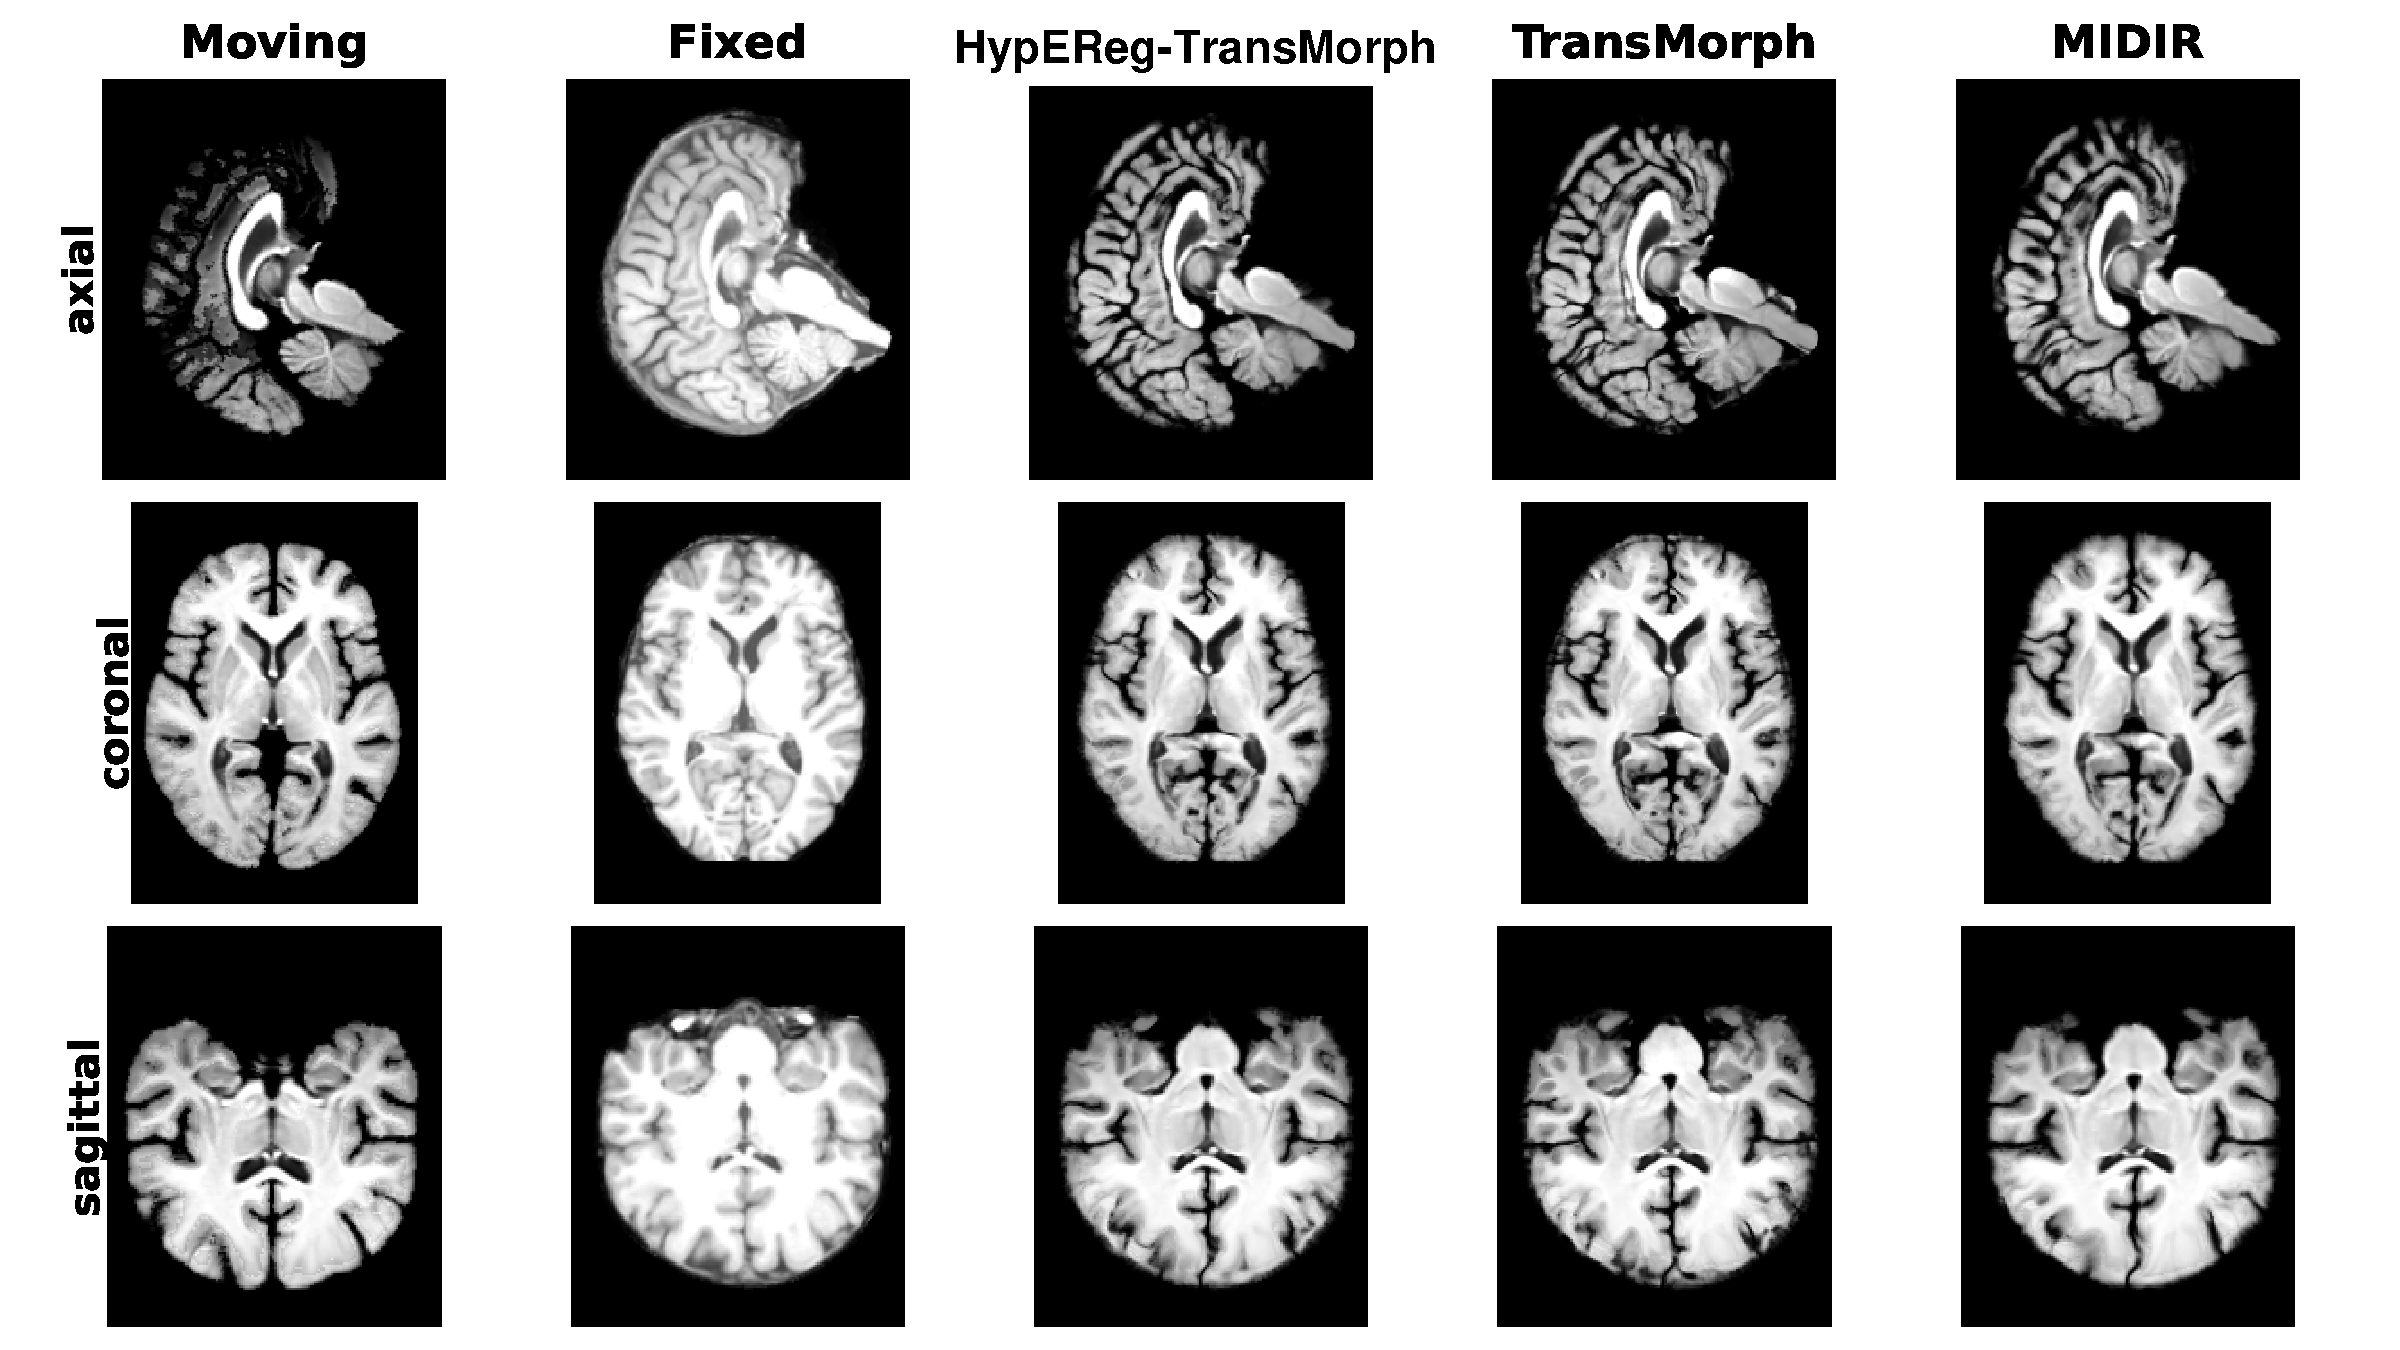
\includegraphics[width=0.96\textwidth]{figures/fig2_qualitative.pdf}
\caption{Qualitative registration comparison on a representative IXI test subject across three orthogonal views (axial/coronal/sagittal). Columns show moving atlas, fixed target, and warped outputs from HypEReg-TransMorph, TransMorph, and MIDIR. Boundary-alignment behaviour in ventricles, cortex, and deep gray structures is highlighted, complementing the quantitative trends reported in Section~\ref{sec:results}. (HER-TransMorph in figure panels denotes HypEReg-TransMorph.) \label{fig2}}
\end{figure}

\begin{figure}[H]
\centering
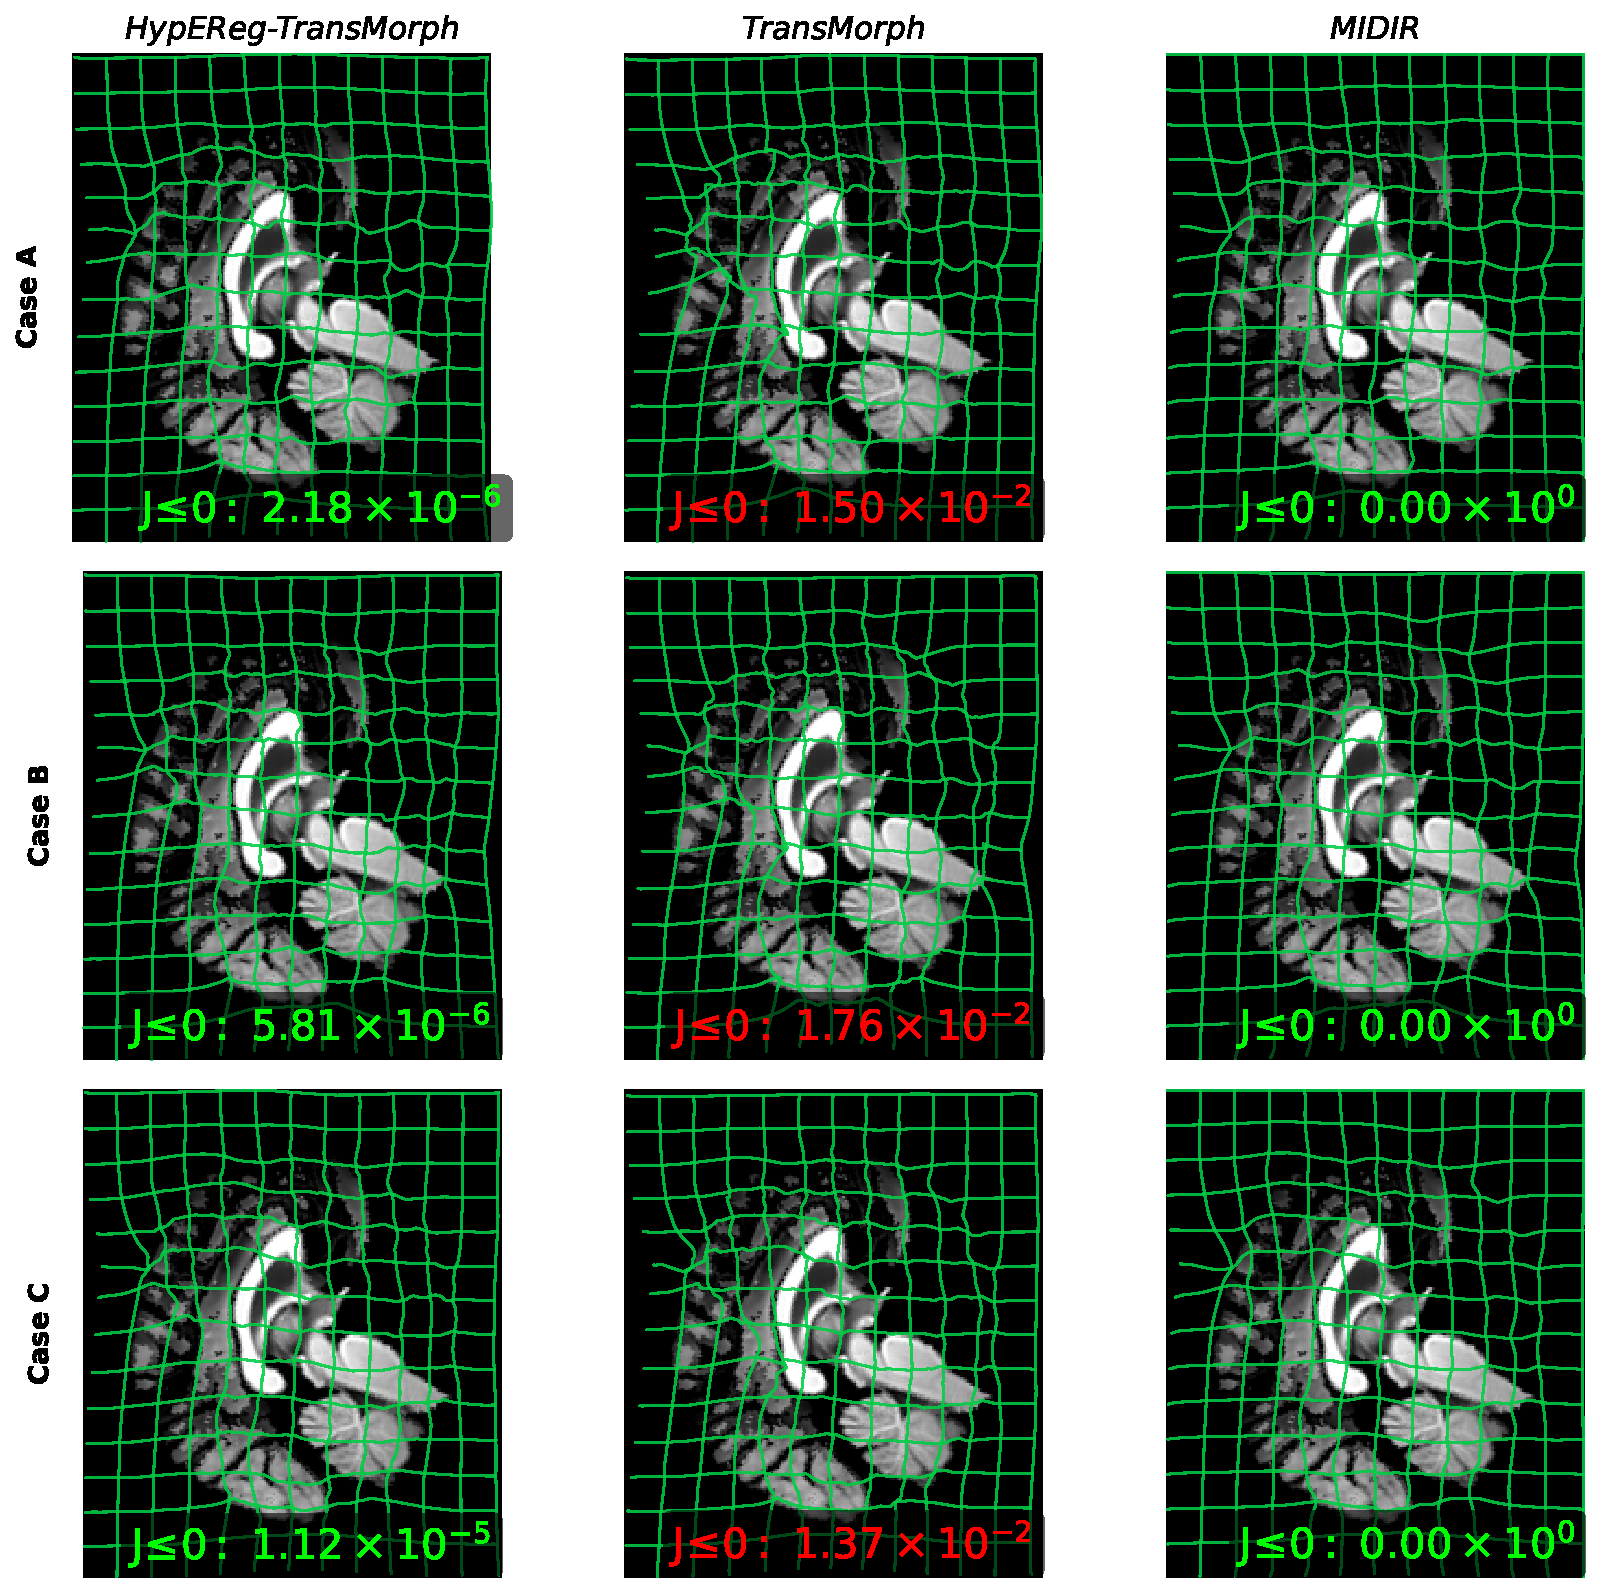
\includegraphics[width=0.96\textwidth]{figures/fig3_gridwarp.pdf}
\caption{Deformation-grid visualization derived from predicted displacement fields on the same IXI subject. Cyan lattice lines represent transformed coordinates after warping by each model. Smooth, non-self-intersecting grids indicate stable local geometry, whereas abrupt kinks or crossings indicate folding risk. In this representative case, HypEReg-TransMorph qualitatively shows smoother global transitions and fewer folding-prone patterns. (HER-TransMorph in figure panels denotes HypEReg-TransMorph.)\label{fig3}}
\end{figure}

%%%%%%%%%%%%%%%%%%%%%%%%%%%%%%%%%%%%%%%%%%
\section{Discussion}\label{sec:discussion}

The present study is positioned as a deformation-quality improvement rather than a contest for the best overlap score. Across the IXI benchmark, HypEReg-TransMorph improves Jacobian regularity and folding suppression---measured by a substantially lower non-positive Jacobian ratio and SDlogJ---while keeping Dice, HD95, and ASSD comparable to or better than strong Transformer baselines. This trade-off is the relevant one for downstream morphometric workflows: high-overlap fields that contain a non-trivial fraction of folded voxels are not directly usable for tensor-based morphometry or atlas-fusion segmentation, regardless of how good the Dice number is.

A natural comparison is the CNN/B-spline baseline MIDIR, which also reaches zero non-positive Jacobian ratio on IXI, with SDlogJ (0.3148) marginally lower than HypEReg-TransMorph (0.3280). The two methods reach comparable regularity through different routes. MIDIR enforces smoothness implicitly via its B-spline parameterization, which structurally rules out folding but also constrains the representational capacity of the warp; HypEReg-TransMorph enforces regularity explicitly through differentiable Jacobian penalties on a dense displacement field, leaving the inference parameterization unchanged. The resulting overlap is higher (Dice 0.7537 vs.\ 0.7423 for MIDIR on IXI), suggesting that explicit Jacobian-determinant control on a dense flow does not necessarily come at a representational cost.

HypEReg also occupies a distinct conceptual position relative to inverse-consistency formulations such as ICON \cite{greer2021icon} and GradICON \cite{tian2023gradicon}, which encourage cycle agreement between forward and inverse warps, and to hierarchical multi-scale constructions such as LapIRN \cite{mok2020lapirn}, which compose deformations across Laplacian pyramids. Inverse consistency and hierarchical composition do not act directly on \(\det J_\phi\); rather, they target different structural properties of the deformation. The constraints are therefore complementary rather than mutually exclusive, and a combined formulation that adds HypEReg on top of an inverse-consistent or hierarchical backbone is a plausible direction for future work.

Within the focused literature on hyperelastic regularization in deep registration, HypEReg differs from existing formulations in three ways. First, the selective Jacobian-determinant penalty of \citet{mok2020fast} contributes only the hinge component of \(\mathcal{L}_{\mathrm{fold}}\); HypEReg adds a non-linear volume-distortion term that controls the entire log-Jacobian distribution rather than only its negative tail. Second, the BMR volume-change-plus-curvature regularizer of \citet{hering2021lung} and the conformal-invariant hyperelastic energy of \citet{zou2023conformal} have been validated only in CNN-based lung-CT pipelines; HypEReg is, to our knowledge, the first non-linear hyperelastic-subset regularizer demonstrated on a Transformer-based dense-flow brain MRI backbone with subject-level paired inferential statistics. Third, by acting directly on \(\det J_\phi\) rather than on first-order strain tensors or conformal-invariant energies, HypEReg targets the geometric quantity that downstream Jacobian-based morphometry actually consumes, and it remains valid at arbitrary local strains rather than approximating a small-strain regime.

The improvements we observe have several concrete implications for medical imaging practice. Lower SDlogJ and a near-zero non-positive Jacobian ratio mean that voxel-wise log-Jacobian maps---used as surrogates of regional atrophy or expansion in tensor-based morphometry---are no longer corrupted by spurious negative-determinant voxels, so longitudinal volume-change estimates around the hippocampus, ventricles, and cortical mantle reflect genuine biological change rather than registration artefacts. This is directly relevant to imaging endpoints in Alzheimer's disease, mild cognitive impairment, multiple sclerosis, and other progressive disorders, where small effect sizes are routinely overwhelmed by registration noise. A fold-free warp also guarantees that label propagation from atlas to subject is one-to-one, the assumption required by atlas-fusion segmentation pipelines used for FreeSurfer-style cortical parcellation, radiotherapy organ-at-risk delineation, and pre-surgical planning of deep-brain-stimulation or epilepsy resection targets. The lower bending energy and near-zero non-positive Jacobian ratio reduce the manual-correction burden on clinical readers in these settings. Combined with the maintained Dice/HD95/ASSD performance and the small forward latency reported in Section~\ref{sec:results} (0.0822\,s per volume on a single Blackwell-class GPU; Table~\ref{tab3}), HypEReg-TransMorph supports both intra-operative use cases (where smooth, invertible deformations are required for accurate landmark warping) and population-scale studies (where thousands of subjects must be processed without manual quality-control flagging of folded fields). Finally, because HypEReg modifies only the loss function and leaves the inference architecture and parameter count unchanged (Table~\ref{tab3}), existing TransMorph-based workflows can adopt it without retraining downstream tools or reconfiguring deployment infrastructure.

Several limitations of the present study should be acknowledged. The headline IXI numbers come from a single training run without a globally pinned random seed; inferential analysis is therefore performed across the 115 held-out test subjects, where the non-parametric paired tests are robust to single-run sampling. The most informative robustness extension is a multi-seed repeat (\(\geq 3\) independent re-trainings of HypEReg-TransMorph and the strongest baselines, with inferential aggregation across subjects and seeds), which the released training scripts already support. The term-by-term ablation in Table~\ref{tab:ablation_terms} is wired for external completion; a server-side run is in progress and the rows will be populated from per-case CSVs in the supplementary release. The clinical evaluation is also indirect: regularity gains have been quantified only at the level of deformation-field metrics, not at the level of biomarker sensitivity or reader workload. Beyond IXI and the OASIS cross-cohort retraining and evaluation reported here, future work will move toward pathology-rich cohorts, LPBA40/Mindboggle-style external benchmarks, multi-modal registration, uncertainty-aware formulations, and adaptive spatially varying hyperelastic weights. Prospective clinical validation on disease-specific cohorts---ADNI for neurodegeneration and BraTS for tumour segmentation are natural starting points---will be needed to quantify how regularity gains translate into biomarker sensitivity and reduced reader workload.

%%%%%%%%%%%%%%%%%%%%%%%%%%%%%%%%%%%%%%%%%%
\section{Conclusions}\label{sec:conclusion}

We have introduced HypEReg, a non-linear hyperelastic regularizer that couples a clamped-rational volume-distortion term with an explicit anti-folding hinge and acts directly on the Jacobian determinant of the predicted displacement field. Integrated into a TransMorph dense-flow backbone, the regularizer produces HypEReg-TransMorph, a learned brain MRI registration model that delivers near-diffeomorphic deformations at zero inference cost. On the IXI atlas-to-subject benchmark with 115 held-out test subjects, HypEReg-TransMorph reduces the non-positive Jacobian-determinant ratio by approximately three orders of magnitude relative to TransMorph and TransMorphBayes (1.502\% \(\to\) 0.0015\%), reduces SDlogJ from 0.5064 to 0.3280, and reduces HD95 from 5.88\,mm to 3.16\,mm, while preserving grouped Dice and adding no inference latency or parameter overhead (Table~\ref{tab3}). A term-by-term ablation isolates the complementary contributions of the volume-distortion and anti-folding penalties (Section~\ref{sec:ablation_terms}; Table~\ref{tab:ablation_terms}), and a strict IXI\(\to\)OASIS zero-shot evaluation confirms that HypEReg-TransMorph attains the highest Dice and the lowest non-positive Jacobian ratio in the zero-shot group---roughly two orders of magnitude below plain TransMorph zero-shot (Section~\ref{sec:oasis_zs}; Table~\ref{tab:oasis_zeroshot}; Figure~\ref{fig:oasis_jacobian}).

These results address a long-standing usability gap of learning-based registration: Jacobian-based biomarkers, atlas-fusion segmentation, and longitudinal morphometry pipelines all assume one-to-one, fold-free warps, an assumption that unconstrained Transformer backbones routinely violate. By delivering near-diffeomorphic fields at feed-forward inference speed and without changes to the deployment architecture, HypEReg-TransMorph is a practical drop-in upgrade for brain-MRI research and clinical-research workflows---atrophy quantification in neurodegenerative disease, atlas-based delineation for radiotherapy and surgical planning, and population-scale morphometry---without sacrificing the throughput and reproducibility advantages that motivated the move from classical iterative methods to learned registration in the first place. With the released open-source package and the planned multi-seed retraining and additional external cohort experiments, non-linear Jacobian-aware regularization is positioned as a low-cost building block for clinically deployable Transformer-based deformable registration.

%%%%%%%%%%%%%%%%%%%%%%%%%%%%%%%%%%%%%%%%%%
\vspace{6pt}

%%%%%%%%%%%%%%%%%%%%%%%%%%%%%%%%%%%%%%%%%%
\supplementary{Supplementary Materials (separate PDF) include: Table~S1 (inferential summary for selected baselines), Table~S2 (paired inferential statistics with Wilcoxon+BH-FDR), Table~S3 (grouped-VOI label mapping), Figure~S1 (descriptive IXI multi-metric overview), OASIS training/environment details, Table~S4 (term-by-term ablation per-case hooks), Table~S5 (OASIS paired Wilcoxon/BH-FDR), implementation and profiling details, and additional qualitative registration/Jacobian visualizations.}

%%%%%%%%%%%%%%%%%%%%%%%%%%%%%%%%%%%%%%%%%%
\authorcontributions{Conceptualization, S.X. and M.X.; methodology, S.X. and M.X.; software, S.X.; validation, S.X. and M.X.; formal analysis, S.X.; investigation, S.X.; data curation, S.X.; writing---original draft preparation, S.X.; writing---review and editing, S.X. and M.X.; visualization, S.X.; supervision, M.X.; project administration, M.X. All authors have read and agreed to the published version of the manuscript.}

\funding{This research received no external funding.}

\institutionalreview{Not applicable. This study performed secondary analysis of publicly available anonymized IXI data and did not recruit new human participants.}

\informedconsent{Not applicable to this secondary-analysis study using publicly available anonymized data.}

\dataavailability{Source code, configuration files, per-case metric tables, and figure/statistics scripts are openly available at \url{https://github.com/Zzxmh/HypEReg-TransMorph} and archived at Zenodo: \url{https://doi.org/10.5281/zenodo.19888526} \cite{xu2026hypereg_zenodo}. Trained model weights are available from the corresponding author upon reasonable request. The IXI dataset used in this study is publicly available at \url{https://brain-development.org/ixi-dataset/} (CC BY-SA 3.0). The preprocessed split follows the public TransMorph-style IXI preprocessing release.}

\acknowledgments{The authors thank Prof.\ Xueqing Yan for academic guidance and computational resource support, and Dr.\ Jiawei Chen for methodological inspiration. The authors also thank the maintainers of open-source registration baselines and the IXI data contributors.}

\conflictsofinterest{The authors declare no conflicts of interest.}

%%%%%%%%%%%%%%%%%%%%%%%%%%%%%%%%%%%%%%%%%%
\abbreviations{Abbreviations}{
The following abbreviations are used in this manuscript:
\\
\noindent
\begin{tabular}{@{}ll}
HypEReg & Hyperelastic-Energy Regularization\\
MRI & Magnetic Resonance Imaging\\
HD95 & 95th percentile Hausdorff Distance\\
ASSD & Average Symmetric Surface Distance\\
NCC & Normalized Cross-Correlation\\
LNCC & Local Normalized Cross-Correlation\\
SDlogJ & Standard Deviation of Log Jacobian Determinant\\
IXI & Information eXtraction from Images dataset\\
BMR & Burger--Modersitzki--Ruthotto (hyperelastic energy framework)\\
FDR & False Discovery Rate
\end{tabular}
}

%%%%%%%%%%%%%%%%%%%%%%%%%%%%%%%%%%%%%%%%%%
\begin{adjustwidth}{-\extralength}{0cm}

\reftitle{References}

%=====================================
% References, variant A: external bibliography
%=====================================
\bibliography{refs}

\end{adjustwidth}
\end{document}

